\documentclass[a4paper,12pt,twoside,scale = 0.8]{report}
\usepackage[left=3cm,right=2.5cm,top=2.8cm,bottom=2.5cm]{geometry}
\usepackage[table]{xcolor}
\usepackage{amssymb}
\usepackage{hyperref}
\usepackage{apacite}
\usepackage{enumitem}
\usepackage{tocbibind}
\usepackage{tikz}
\usepackage{graphicx}
\usepackage{indentfirst} 
\usepackage{amsmath}
\usepackage{amsfonts}
\usepackage{amssymb}
\usepackage{epstopdf}
\usepackage{cleveref}
\usepackage{float}
\usepackage{parskip}
%\usepackage{setspace}
\usepackage{natbib}
\usepackage{booktabs}
\usepackage{makecell}
\usepackage{caption}
\usepackage{titlesec}
\usepackage{nomencl}
\usepackage{bm}
\usetikzlibrary{matrix}
\usepackage{adjustbox}
\usetikzlibrary{positioning}
\usepackage[sort=use,acronym]{glossaries}



\makeglossaries
\makenomenclature

\crefname{figure}{Figure}{Figures}
\crefname{equation}{Equation}{Equations}

\usepackage{geometry}
\geometry{includeheadfoot,left=1in,right=1in,top=1cm,bottom=1cm,asymmetric,bindingoffset=0pt,nomarginpar}
\usepackage[table]{xcolor}
\usepackage{amssymb}
\usepackage[final]{hyperref}
\usepackage{apacite}
\usepackage{enumitem}
\usepackage{tikz}
\usepackage{graphicx}
\usepackage{indentfirst} 
\usepackage{amsmath}
\usepackage{amsfonts}
\usepackage{amssymb}
\usepackage{epstopdf}
\usepackage{cleveref}
\usepackage{float}
\usepackage{parskip}
%\usepackage{setspace}
\usepackage{natbib}
\usepackage{booktabs}
\usepackage{makecell}
\usepackage{caption}
\usepackage{titlesec}
\usepackage[intoc]{nomencl}
\usepackage{bm}
\usetikzlibrary{matrix}
\usepackage{adjustbox}
\usetikzlibrary{positioning}
\usepackage[toc,acronym]{glossaries}
\usepackage{graphicx}
\usepackage{verbatim}
\usepackage{latexsym}
\usepackage{mathchars}
\usepackage{setspace}
\usepackage{emptypage}
\usepackage{tocbibind}
\usepackage{etoc}
\usepackage{multicol}
\usepackage{glossary-mcols}
\usepackage{amssymb}
\usepackage[ruled,longend,linesnumbered]{algorithm2e}
\usepackage{cleveref}
\usepackage{xr-hyper}
\usepackage{subcaption}
\renewcommand*{\algorithmcfname}{}
\renewcommand{\thealgocf}{Algorithm \ \arabic{algocf}}

\raggedbottom
%\renewcommand\nompreamble{\begin{multicols}{2}}
%\renewcommand\nompostamble{\end{multicols}}
%\renewcommand\acrpreamble{\begin{multicols}{2}}
%\renewcommand\acrpostamble{\end{multicols}}

\hypersetup{
    colorlinks=true,
    linkcolor=blue,
    citecolor=blue,
    urlcolor=blue}

\makeglossaries
\makenomenclature

\crefname{figure}{Figure}{Figures}
\crefname{equation}{Equation}{Equations}

\titlespacing{\chapter}{0pt}{\dimexpr\parskip-1ex}{\dimexpr\parskip-0.5ex}
\titlespacing{\section}{0pt}{\dimexpr\parskip-0.5ex}{\dimexpr\parskip-0.25ex}
\titlespacing{\subsection}{0pt}{\dimexpr\parskip-0.25ex}{\dimexpr\parskip-0.5ex}

%\setlength{\intextsep}{10pt}

\setlength{\parskip}{\medskipamount}  % a little space before a \par
\setlength{\parindent}{0pt}	      % don't indent first lines of paragraphs
%UHEAD.STY  If this is included after \documentstyle{report}, it adds
% an underlined heading style to the LaTeX report style.
% \pagestyle{uheadings} will put underlined headings at the top
% of each page. The right page headings are the Chapter titles and
% the left page titles are supplied by \def\lefthead{text}.

% Ted Shapin, Dec. 17, 1986

\makeatletter
\def\chapapp2{Chapter}

\def\appendix{\par
 \setcounter{chapter}{0}
 \setcounter{section}{0}
 \def\chapapp2{Appendix}
 \def\@chapapp{Appendix}
 \def\thechapter{\Alph{chapter}}}

\def\ps@uheadings{\let\@mkboth\markboth
% modifications
\def\@oddhead{\protect\underline{\protect\makebox[\textwidth][l]
		{\sl\rightmark\hfill\rm\thepage}}}
\def\@oddfoot{}
\def\@evenfoot{}
\def\@evenhead{\protect\underline{\protect\makebox[\textwidth][l]
		{\rm\thepage\hfill\sl\leftmark}}}
% end of modifications
\def\chaptermark##1{\markboth {\ifnum \c@secnumdepth >\m@ne
 \chapapp2\ \thechapter. \ \fi ##1}{}}%
\def\sectionmark##1{\markright {\ifnum \c@secnumdepth >\z@
   \thesection. \ \fi ##1}}}
\makeatother
%%From: marcel@cs.caltech.edu (Marcel van der Goot)
%%Newsgroups: comp.text.tex
%%Subject: illegal modification of boxit.sty
%%Date: 28 Feb 92 01:10:02 GMT
%%Organization: California Institute of Technology (CS dept)
%%Nntp-Posting-Host: andromeda.cs.caltech.edu
%%
%%
%%Quite some time ago I posted a file boxit.sty; maybe it made it
%%to some archives, although I don't recall submitting it. It defines
%%	\begin{boxit}
%%	...
%%	\end{boxit}
%%to draw a box around `...', where the `...' can contain other
%%environments (e.g., a verbatim environment). Unfortunately, it had
%%a problem: it did not work if you used it in paragraph mode, i.e., it
%%only worked if there was an empty line in front of \begin{boxit}.
%%Luckily, that is easily corrected.
%%
%%HOWEVER, apparently someone noticed the problem, tried to correct it,
%%and then distributed this modified version. That would be fine with me,
%%except that:
%%1. There was no note in the file about this modification, it only has my
%%   name in it.
%%2. The modification is wrong: now it only works if there is *no* empty
%%   line in front of \begin{boxit}. In my opinion this bug is worse than
%%   the original one.
%%
%%In particular, the author of this modification tried to force an empty
%%line by inserting a `\\' in the definition of \Beginboxit. If you have
%%a version of boxit.sty with a `\\', please delete it. If you have my
%%old version of boxit.sty, please also delete it. Below is an improved
%%version.
%%
%%Thanks to Joe Armstrong for drawing my attention to the bug and to the
%%illegal version.
%%
%%                                          Marcel van der Goot
%% .---------------------------------------------------------------
%% | Blauw de viooltjes,                    marcel@cs.caltech.edu
%% |    Rood zijn de rozen;
%% | Een rijm kan gezet
%% |    Met plaksel en dozen.
%% |


% boxit.sty
% version: 27 Feb 1992
%
% Defines a boxit environment, which draws lines around its contents.
% Usage:
%   \begin{boxit}
%	... (text you want to be boxed, can contain other environments)
%   \end{boxit}
%
% The width of the box is the width of the contents.
% The boxit* environment behaves the same, except that the box will be
% at least as wide as a normal paragraph.
%
% The reason for writing it this way (rather than with the \boxit#1 macro
% from the TeXbook), is that now you can box verbatim text, as in
%   \begin{boxit}
%   \begin{verbatim}
%   this better come out in boxed verbatim mode ...
%   \end{verbatim}
%   \end{boxit}
%
%						Marcel van der Goot
%						marcel@cs.caltech.edu
%

\def\Beginboxit
   {\par
    \vbox\bgroup
	   \hrule
	   \hbox\bgroup
		  \vrule \kern1.2pt %
		  \vbox\bgroup\kern1.2pt
   }

\def\Endboxit{%
			      \kern1.2pt
		       \egroup
		  \kern1.2pt\vrule
		\egroup
	   \hrule
	 \egroup
   }	

\newenvironment{boxit}{\Beginboxit}{\Endboxit}
\newenvironment{boxit*}{\Beginboxit\hbox to\hsize{}}{\Endboxit}
\pagestyle{empty}

\setlength{\parskip}{2ex plus 0.5ex minus 0.2ex}
\setlength{\parindent}{2em}

% \titlespacing{\section}{0pt}{\parskip}{-\parskip}
% \titlespacing{\subsection}{0pt}{\parskip}{-\parskip}
\makeatletter  %to avoid error messages generated by "\@". Makes Latex treat "@" like a letter

\linespread{1.5}
\def\submitdate#1{\gdef\@submitdate{#1}}

\def\maketitle{
  \begin{titlepage}{
    %\linespread{1.5}
    \Large University of London \\
    %\linebreak
    Imperial College of Science, Technology and Medicine \\
    %\linebreak
    Department of Civil and Environmental Engineering
    \rm
    \vskip 3in
    \Large \bf \@title \par
  }
  \vskip 0.3in
  \par
  {\Large \@author}
  \vskip 4in
  \par
  Submitted on \today
  \vfil
  \end{titlepage}
}

\def\titlepage{
  \newpage
  \centering
  \linespread{1}
  \normalsize
  \vbox to \vsize\bgroup\vbox to 9in\bgroup
}
\def\endtitlepage{
  \par
  \kern 0pt
  \egroup
  \vss
  \egroup
  \cleardoublepage
}

\def\abstract{
  \begin{center}{
    \large\bf Abstract}
  \end{center}
  \small
  %\def\baselinestretch{1.5}
  \linespread{1.5}
  \normalsize
}
\def\endabstract{
  \par
}

\newenvironment{acknowledgements}{
  \cleardoublepage
  \begin{center}{
    \large \bf Acknowledgements}
  \end{center}
  \small
  \linespread{1.5}
  \normalsize
}{\cleardoublepage}
\def\endacknowledgements{
  \par
}

\newenvironment{dedication}{
  \cleardoublepage
  \begin{center}{
    \large \bf Dedication}
  \end{center}
  \small
  \linespread{1.5}
  \normalsize
}{\cleardoublepage}
\def\enddedication{
  \par
}

\def\preface{
    \pagenumbering{roman}
    \pagestyle{plain}
    \doublespacing
}


\def\body{
    \cleardoublepage    
    \pagestyle{uheadings}
    \tableofcontents
    \pagestyle{plain} 
    \cleardoublepage
    \pagestyle{uheadings}
    \listoftables
    \pagestyle{plain}
    \cleardoublepage
    \pagestyle{uheadings}
    \listoffigures
    \pagestyle{plain}
    \cleardoublepage
    \pagestyle{uheadings}
    \pagenumbering{arabic}
    \doublespacing
}

\makeatother  %to avoid error messages generated by "\@". Makes Latex treat "@" like a letter

\newcommand{\ipc}{{\sf ipc}}

\newcommand{\Prob}{\bbbp}
\newcommand{\Real}{\bbbr}
\newcommand{\real}{\Real}
\newcommand{\Int}{\bbbz}
\newcommand{\Nat}{\bbbn}

\newcommand{\NN}{{\sf I\kern-0.14emN}}   % Natural numbers
\newcommand{\ZZ}{{\sf Z\kern-0.45emZ}}   % Integers
\newcommand{\QQQ}{{\sf C\kern-0.48emQ}}   % Rational numbers
\newcommand{\RR}{{\sf I\kern-0.14emR}}   % Real numbers
\newcommand{\KK}{{\cal K}}
\newcommand{\OO}{{\cal O}}
\newcommand{\AAA}{{\bf A}}
\newcommand{\HH}{{\bf H}}
\newcommand{\II}{{\bf I}}
\newcommand{\LL}{{\bf L}}
\newcommand{\PP}{{\bf P}}
\newcommand{\PPprime}{{\bf P'}}
\newcommand{\QQ}{{\bf Q}}
\newcommand{\UU}{{\bf U}}
\newcommand{\UUprime}{{\bf U'}}
\newcommand{\zzero}{{\bf 0}}
\newcommand{\ppi}{\mbox{\boldmath $\pi$}}
\newcommand{\aalph}{\mbox{\boldmath $\alpha$}}
\newcommand{\bb}{{\bf b}}
\newcommand{\ee}{{\bf e}}
\newcommand{\mmu}{\mbox{\boldmath $\mu$}}
\newcommand{\vv}{{\bf v}}
\newcommand{\xx}{{\bf x}}
\newcommand{\yy}{{\bf y}}
\newcommand{\zz}{{\bf z}}
\newcommand{\oomeg}{\mbox{\boldmath $\omega$}}
\newcommand{\res}{{\bf res}}
\newcommand{\cchi}{{\mbox{\raisebox{.4ex}{$\chi$}}}}
%\newcommand{\cchi}{{\cal X}}
%\newcommand{\cchi}{\mbox{\Large $\chi$}}

% Logical operators and symbols
\newcommand{\imply}{\Rightarrow}
\newcommand{\bimply}{\Leftrightarrow}
\newcommand{\union}{\cup}
\newcommand{\intersect}{\cap}
\newcommand{\boolor}{\vee}
\newcommand{\booland}{\wedge}
\newcommand{\boolimply}{\imply}
\newcommand{\boolbimply}{\bimply}
\newcommand{\boolnot}{\neg}
\newcommand{\boolsat}{\!\models}
\newcommand{\boolnsat}{\!\not\models}


\newcommand{\op}[1]{\mathrm{#1}}
\newcommand{\s}[1]{\ensuremath{\mathcal #1}}

% Properly styled differentiation and integration operators
\newcommand{\diff}[1]{\mathrm{\frac{d}{d\mathit{#1}}}}
\newcommand{\diffII}[1]{\mathrm{\frac{d^2}{d\mathit{#1}^2}}}
\newcommand{\intg}[4]{\int_{#3}^{#4} #1 \, \mathrm{d}#2}
\newcommand{\intgd}[4]{\int\!\!\!\!\int_{#4} #1 \, \mathrm{d}#2 \, \mathrm{d}#3}

% Large () brackets on different lines of an eqnarray environment
\newcommand{\Leftbrace}[1]{\left(\raisebox{0mm}[#1][#1]{}\right.}
\newcommand{\Rightbrace}[1]{\left.\raisebox{0mm}[#1][#1]{}\right)}

% Funky symobols for footnotes
\newcommand{\symbolfootnote}{\renewcommand{\thefootnote}{\fnsymbol{footnote}}}
% now add \symbolfootnote to the beginning of the document...

\newcommand{\normallinespacing}{\renewcommand{\baselinestretch}{1.5} \normalsize}
\newcommand{\mediumlinespacing}{\renewcommand{\baselinestretch}{1.2} \normalsize}
\newcommand{\narrowlinespacing}{\renewcommand{\baselinestretch}{1.0} \normalsize}
\newcommand{\bump}{\noalign{\vspace*{\doublerulesep}}}
\newcommand{\cell}{\multicolumn{1}{}{}}
\newcommand{\spann}{\mbox{span}}
\newcommand{\diagg}{\mbox{diag}}
\newcommand{\modd}{\mbox{mod}}
\newcommand{\minn}{\mbox{min}}
\newcommand{\andd}{\mbox{and}}
\newcommand{\forr}{\mbox{for}}
\newcommand{\EE}{\mbox{E}}

\newcommand{\deff}{\stackrel{\mathrm{def}}{=}}
\newcommand{\syncc}{~\stackrel{\textstyle \rhd\kern-0.57em\lhd}{\scriptstyle L}~}

\def\coop{\mbox{\large $\rhd\!\!\!\lhd$}}
\newcommand{\sync}[1]{\raisebox{-1.0ex}{$\;\stackrel{\coop}{\scriptscriptstyle
#1}\,$}}

\newtheorem{definition}{Definition}[chapter]
\newtheorem{theorem}{Theorem}[chapter]

\newcommand{\Figref}[1]{Figure~\ref{#1}}
\newcommand{\fig}[3]{
 \begin{figure}[!ht]
 \begin{center}
 \scalebox{#3}{\includegraphics{figs/#1.ps}}
 \vspace{-0.1in}
 \caption[ ]{\label{#1} #2}
 \end{center}
 \end{figure}
}

\newcommand{\figtwo}[8]{
 \begin{figure}
 \parbox[b]{#4 \textwidth}{
 \begin{center}
 \scalebox{#3}{\includegraphics{figs/#1.ps}}
 \vspace{-0.1in}
 \caption{\label{#1}#2}
 \end{center}
 }
 \hfill
 \parbox[b]{#8 \textwidth}{
 \begin{center}
 \scalebox{#7}{\includegraphics{figs/#5.ps}}
 \vspace{-0.1in}
 \caption{\label{#5}#6}
 \end{center}
 }
 \end{figure}
}
\titlespacing{\chapter}{0pt}{\dimexpr\parskip-1ex}{\dimexpr\parskip-0.5ex}
\titlespacing{\section}{0pt}{\dimexpr\parskip-0.5ex}{\dimexpr\parskip-0.25ex}
\titlespacing{\subsection}{0pt}{\dimexpr\parskip-0.25ex}{\dimexpr\parskip-0.5ex}





\begin{document}

\title{\LARGE {\bf Data-driven uncertainty quantification and predictive digital twin for offshore piles}\\
 \vspace*{6mm}
}

\author{Ningxin Yang}
\submitdate{October 2008}

\normallinespacing
\maketitle

%\preface
\begin{abstract}

The identification of representative parameters is an essential component in performing numerical modelling of geostructures. Uncertainties in the geotechnical context arise from several factors, such as differences between in-situ tests and laboratory conditions, spatial variations in the soil profile, and the choices of the constitutive model. Numerical modelling of geostructures is further complicated by uncertainties resulting from the choice of stages construction or complex physics. Traditional methods of manual back analysis or probabilistic design methods based on Monte Carlo simulation to understand the inherent variability in the ground are either time-consuming or computationally expensive. A Bayesian probabilistic framework offers an alternative approach to both manual and Monte Carlo type back-analysis for ground characterisation. The approach offers a mathematically robust framework for incorporating prior knowledge and data assimilation.

Nowadays, data-driven methodologies have permeated various engineering domains. However, in the realm of geotechnical engineering, there exists a notable absence of guidelines for data-driven uncertainty quantification (UQ). This thesis endeavors to address this gap by delving into the latest research and hopes to put forth a comprehensive UQ design framework that can be generally applied in geotechnical engineering. The efficacy of the proposed framework will be assessed by comparing the data-driven inferred soil parameters against those obtained by manual back-analysis. As a first step, this thesis will present the results and findings relevant to the PISA project, a combined field testing and numerical modelling study into the design of piles subjected to lateral loading, with the aim of developing a comprehensive data set for applying the data-driven uncertainty quantification approach.



\end{abstract}
%\cleardoublepage

\addcontentsline{toc}{chapter}{Acknowledgements}

\begin{acknowledgements}

I would like to express (whatever feelings I have) to:

\begin{itemize}
 \item My supervisor: Dr Truong Le
 \vspace*{3mm}
 \item My second supervisor: Prof. Lidija Zdravkovic

 \vspace*{3mm}
 \item Other researchers
 \vspace*{3mm}
 \item My family and friends
\end{itemize}

\end{acknowledgements}
%\cleardoublepage

% \begin{dedication}
%   Dedication here.
% \end{dedication}
%\clearpage

\narrowlinespacing

\vspace*{4mm}

`Quote text here.'\\
\\
\emph{Guy Quoted}

\normallinespacing

\body
\clearpage
\addcontentsline{toc}{chapter}{Nomenclature}


\nomenclature{$\mathcal{M}$}{Computational model\hfill}
\nomenclature{$\bm{y}$}{Model response\hfill}
\nomenclature{$\bm{x}$}{Vector of input parameter\hfill}
\nomenclature{$\mathcal{M}_{d}(\bm{x})$}{Deterministic output\hfill}
\nomenclature{$\mathcal{M}_{s}(\bm{x})$}{Stochastic output\hfill}
\nomenclature{$\tilde{\mathcal{M}}_{d}$}{Surrogate model\hfill}   
\nomenclature{$\mathcal{M}_{d}$}{Deterministic simulator\hfill}
\nomenclature{$\mathcal{M}_{s}$}{Stochastic simulator\hfill}
\nomenclature{$\mathcal{D}_{\bm{X}}$}{Input parameters space\hfill}  
\nomenclature{$\mathcal{\bm{X}}$}{Experimental design\hfill}
\nomenclature{$\varepsilon$}{Generalization error\hfill}



\printnomenclature[1in]
\clearpage
\addcontentsline{toc}{chapter}{Acronyms}


\newacronym{MCMC}{MCMC}{Markov Chain Monte Carlo}
\newacronym{PDF}{PDF}{Probability Density Function}
\newacronym{MAP}{MAP}{maximum a posterior}


\printglossary[type=\acronymtype]
% body of thesis comes here
\chapter{Introduction}
\label{intro}

\section{Background}

Offshore monopiles are increasingly preferred for wind farm installations, owing to their benefits in clean energy generation and convenient deployment. These cylindrical steel structures are driven into the seabed to establish a stable foundation for wind turbines. While offshore wind energy holds promise as a source of clean and sustainable power, the adoption of offshore monopiles introduces specific engineering challenges. A primary concern associated with offshore monopiles is addressing potential issues related to excessive pile displacements induced during both their installation and operation phases \citep{byrne2003,randolph2005}. Excessive movements in the piles can result in significant displacements and rotations within supporting structures, subsequently leading to damage or structural instability. The accurate prediction and effective management of pile deformations is therefore of paramount when designing and analyzing support systems for offshore monopile installations.





Design loads and pile dimensions are most often acquired from a technical report. These are typically developed by either empirical solutions presented in guidelines or by using numerical simulations. Several design methods have been provided in the design codes \citep{api2011,bhattacharya2019} to predict offshore pile $p-y$ curve. However, it is still a challenge to incorporate all influential factors, such as pile length, soil layer, soil properties and loading conditions, into a simplified empirical model. Rapid advancement in efficiency and power of computational techniques has opened the potential for numerical models to be used as a design tool \citep{randolph2017,taborda2020,zdravkovic2020,royston2022}. Unfortunately, in order to perform robust forward analysis, a substantial number of simulations must be run to capture the spatial uncertainty of the problem. This presents a significant challenge for the back-analysis of the parameters, especially in the context of inverse and predictive analysis.

In recent research endeavors, Bayesian probability frameworks have garnered increasing recognition as an efficacious approach for inverse parameter estimation and response prediction \citep{finno2005,nakamura2011,hsein2013,nguyen2016,wagner2020,jin2021,tao2021,buckley2023,tang2023}. In such circumstances, the Bayesian framework emerges as a powerful tool within the probabilistic context, facilitating parameter learning and informed decision-making. However, for high fidelity numerical models used in geotechnical engineering, the computational cost of completing these analyses can be very expensive. Traditional Monte Carlo methods for UQ or manually overcoming this limitation is often not feasible. There is an urgent requirement to tackle these issues. Fortunately, significant research has been undertaken in the UQ and machine learning domain to address issues related to large-scale data models and uncertainty. However, in geotechnical engineering, there is a noticeable absense of guidlines for UQ area. This research attempts to bridge this gap by developing a data-driven dynamic UQ framework. 

In practice, through adaptive Bayesian updating on the identified parameters and reduce the uncertainties on offshore piles, a field engineer would benefit from: (1) properly accounting the uncertainties of input variables; (2) real-time monitoring and adaptively predicting the pile response in probabilistic setting; (3) providing an efficient tool for data-driven decision making on pile operation and design. In the context of offshore engineering, the approach has significant potentials in several domains. This includes, but not limited to health monitoring, pile penetration and long-term bearing capacities \citep{wang2021,zhao2023,stuyts2023}. 



\section{Problem statement}

Modern pile installation and proper estimation is becoming increasingly complex and vital to the reliability and permanence of the foundation in question. However, in the construction process, poor understanding of the soil physics, combined with our inability to model complex boundary/soil conditions lead to inaccurate predictions of pile responses. The source of uncertainties may come from various reasons. Dealing with different uncertainties sources is a challenging task. One typical uncertainty source can be illustrated in \cref{fig: Cowden_cpt}, which shows parts of uncertainties sources:

% \setlength{\parskip}{0pt}
% \setlist[itemize]{itemsep=0pt,topsep=0pt,parsep=0pt,partopsep=0pt}

\begin{itemize}[left=0pt]

    \item Fluctuating curve indicates the spatial variability
    \item Non-uniformity exists between in-situ test and laboratory experiment

\end{itemize}
\vspace{0.2cm}


In engineering applications, uncertainty quantification (UQ) often involves simulations with a large number of input parameters. Some well-established approaches are proposed for fitting pile deformations to infer the underlying soil parameters and reduce uncertainties. However, addressing uncertainties based on traditional \textit{Monte Carlo} methods in such systems can be computationally intensive. In these scenarios, it becomes practical to replace the computational model with a surrogate.  A surrogate model $\tilde{\mathcal{M}}$ can be then expressed as:
\begin{equation}
\label{eq:surrogate_model}
    \tilde{\mathcal{M}}(\boldsymbol{X})  \overset{\mathrm{def}}{=} \mathcal{M}(\boldsymbol{X}) - \mathcal{R}(\boldsymbol{X})
\end{equation}
where $\mathcal{R}$ is the residual between the original model and the surrogate. Nevertheless, as dimensions increase, the efficacy of surrogate models diminishes, accompanied by escalating computational and storage expenses. This is widely acknowledged as the \textit{curse of dimensionality} \citep{verleysen2005}. 


\begin{figure}[htbp]
    \center
    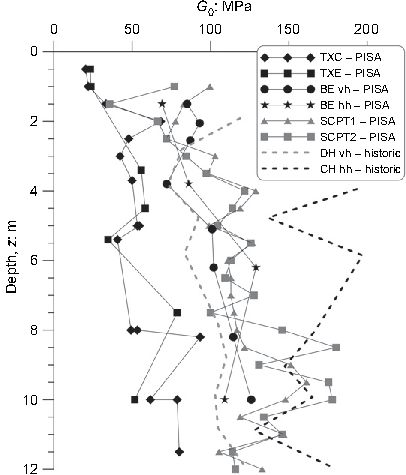
\includegraphics[width = 90mm]{Figures/figure-Cowden.pdf}
    \caption{Stiffness characteristics at Cowden from \protect\cite{zdravkovic2020}}
    \label{fig: Cowden_cpt}
\end{figure}






\section{Objectives and outlines}
\subsubsection{Objectives:}
This thesis aims to construct a robust and scalable framework for uncertainty quantification, extending its applicability beyond offshore piles. This endeavor will leverage cutting-edge methodologies in the fields of surrogate modeling, uncertainty quantification, probabilistic graphical model and control theory, to deliver a robust digital twin framework in geotechnical engineering. In particular, the specific goals of this research are:
\begin{itemize}[left=0pt]
    \item Develop a surrogate model suitable, not limited for offshore piles, for structures characterized by high input dimensions.
    
    \item Accelerate Bayesian inversion calculations for identified parameters to reduce the uncertainties, and providing real-time response predictions through adaptive enrichment of observed monitoring data.
    
    \item Develop an adaptive uncertainty quantification framework.

  
\end{itemize}


\subsubsection{Outlines:}
Chapter 2 introduces the fundamentals of Bayesian probabilistic theory.
Chapter 3 discusses the most important forward and inverse UQ tools.
Chapter 4 states the geotechnical UQ problems in our thesis and work plans for the next stage.

\chapter{Bayesian probabilistic theory}


In probabilistic theory, two main interpretations prevail: frequentist and Bayesian. The frequentist perspective views probabilities as the long-term frequencies observed in infinite trials. For example, in this context, the statement implies that, over many coin flips, heads are expected roughly half the time.

On the other hand, the Bayesian interpretation associates probability with uncertainty and information, rather than repeated trials. From the Bayesian viewpoint, the statement suggests an equal likelihood of the coin landing heads or tails in the next toss.

Depending on the amount of available data, which may range from zero to infinite, various techniques may be used:

\begin{itemize}[left=0pt]
 \item when no data is available to characterize the input parameters, a probabilistic model may be prescribed purely by expert judgment;
 \item when a large amount of data is available, the tools of statistical inference may be fully applied, like the method of moments \citep{wagner2020};
 \item when both expert judgment and very limited observations are available, Bayesian inference may be resorted to.
\end{itemize}

One big advantage of the Bayesian interpretation is that it can be used to model our events that do not have long term frequencies. Take, for example, the assessment of the probability of structural damage to a high-rise building, the collapse of a tunnel, or the occurrence of irreversible deformation in bridge piers.This event is anticipated to occur only a limited number of times over the structure's lifetime and is not expected to happen repeatedly. Nevertheless, we ought to be able to quantify our uncertainty about this event and take appropriate actions (see chapter \ref{UQ} and chapter \ref{DT}).

Since data collection is inherently constrained during the progression of most engineering projects, Bayesian theory stands out as a highly effective method. Therefore, this thesis exclusively explores Bayesian methods next, while detailed information on frequentist approaches can be found in \cite{murphy2012}.



\label{ch:Bayesian}


\section{Bayesian inference}

When dealing with a limited number of data points, direct statistical estimation becomes unreliable due to substantial statistical uncertainty in the sample estimates. In this context, $\textit{Bayesian inference}$ provides a solution by integrating prior knowledge on parameters with a small set of observed data points. Operating in this fully probabilistic setting, all unknowns are treated as random vectors. Distribution parameters can be denoted by $\boldsymbol{x}$ as realisations of the random vector $\boldsymbol{X}:\Omega \rightarrow \mathcal{D}_{\boldsymbol{X}}$. \textit{Quantities of interest} gathered from output are gathered in a vector $\boldsymbol{y} \in \mathbb{R}^{N_{\rm{out}}}$. The joint probability distribution of the combined random vector $(\boldsymbol{X},\boldsymbol{Y}):\Omega \rightarrow \mathcal{D}_{\boldsymbol{X}} \times {D}_{\boldsymbol{Y}}$ is represented by $\pi(\boldsymbol{x};\boldsymbol{y})$. Leveraging the fundamental \textit{sum rule} and \textit{product rule} in probabilistic theory, the \acrfull{PDF} of the parameters and the data can be expressed as
\begin{equation}
\pi(\boldsymbol{x}|\boldsymbol{y}) = \frac{{\mathcal{L}(\boldsymbol{x};\boldsymbol{y}) \cdot \pi(\boldsymbol{x})}}{{\pi(\boldsymbol{y})}} \label{equation Bayes}
\end{equation}
which is also known as \textit{Bayes' theorem} or \textit{Bayes' rule}. In Bayesian terminology, this distribution $\pi(\boldsymbol{x}|\boldsymbol{y})$ is called the posterior distribution and it is calculated by prior $\pi(\boldsymbol{x})$, likelihood $\mathcal{L}(\boldsymbol{x};\boldsymbol{y})\stackrel{\mathrm{def}}{=}\pi(\boldsymbol{y}|\boldsymbol{x})$
and the evidence $\pi(\boldsymbol{y})$. These definitions of the likelihood function and evidence strictly hold only for a single data point $\mathcal{Y}=\{\boldsymbol{y} \}$, but can be generalised to multiple data points easily $\mathcal{Y} \stackrel{\mathrm{def}}{=} \{{\boldsymbol{y}^{(1)}},\cdots,{\boldsymbol{y}^{(N)}}\}$. These terms in \cref{equation Bayes} have practical significance that we will briefly summarise next.
\begin{itemize}[left=0pt]
    \item \textcolor{blue}{Prior $\pi(\boldsymbol{x})$}: In the Bayesian paradigm, before considering the data the parameters $\boldsymbol{x}$ are treated as realisations from a random vector $\boldsymbol{X}$ which is assumed to follow the so-called prior distribution.
    

    \item \textcolor{blue}{Likelihood function $\mathcal{L}(\boldsymbol{x};\mathcal{Y})$}: The likelihood function is a measure of how well the prescribed parametric distribution $\pi(\mathcal{Y}|\boldsymbol{x})$ describes the data. In most engineering cases, input parameters $\boldsymbol{x}$ are not measurable directly. To evaluate the likelihood $\mathcal{L}(\boldsymbol{x};\mathcal{Y})$, some ingredients are needed: a computational forward model $\mathcal{M}$, a set of input parameters $\boldsymbol{x} \in\mathcal{D}_{\boldsymbol{X}}$ that need to be inferred, and a set of experimental data $\mathcal{Y}$.
    The forward model $\boldsymbol{x} \rightarrow \boldsymbol{M}(\boldsymbol{x})$ is a mathematical representation of the system under consideration. All models are always simplifications of the real world. Thus, to connect model predictions to the observations $\mathcal{Y}$, a \textit{discrepancy term} $\boldsymbol{\varepsilon}$ shall be introduced. We consider the following well-established format:
    \begin{equation}
        \label{eq: discrepancy term}
        \boldsymbol{y} = \mathcal{M}(\boldsymbol{x}) + \boldsymbol{\varepsilon}
    \end{equation}
    where $\boldsymbol{\varepsilon} \in \mathbb{R}^{N_{\rm{out}}}$ is the term that describes the discrepancy between an experimental observation $\mathcal{Y}$ and the model prediction. For the sake of simplicity, we consider it as an additive \textit{Gaussian discrepancy} with zero mean and a covariance matrix $\boldsymbol{\Sigma}$ in this introduction:
        \begin{equation}
            \label{eq: Gaussian discrepancy}
            \boldsymbol{\varepsilon} \in \mathcal{N}(\varepsilon|\boldsymbol{0},\boldsymbol{\Sigma})
        \end{equation}
    It is noted that simple Gaussian discrepancy assumption is only one out of many possible models. In a more general setting, other distributions for the discrepancy are used as well \citep{UQdoc}. Due to the widespread used of the additive Gaussian models in engineering disciplines, the thesis is limited to Gaussian type. If $N$ independent measurement $\boldsymbol{y_{i}}$ are available and gathered in the data set $\mathcal{Y} \stackrel{\mathrm{def}}{=} \{{\boldsymbol{y}^{(1)}},\cdots,{\boldsymbol{y}^{(N)}}\}$, the likelihood can thus be written as:
        \begin{equation}        
        \label{eq: Likelihood function}
        \begin{aligned}
         \mathcal{L}(\boldsymbol{x};\mathcal{Y}) =& \prod_{i=1}^{N} N(\boldsymbol{y_{i}}|\mathcal{M}(\boldsymbol{x}),\boldsymbol{\Sigma}) \\
         =& \prod_{i=1}^{N}\frac{1}{\sqrt{(2 \pi)^{N_{\rm{out}}}{\rm{det}} 
         (\boldsymbol{\Sigma})}}\exp\left(-\frac{1}{2}\left(\boldsymbol{y_i} - \mathcal{M}(\boldsymbol{x})\right)^{\mathsf{T}} \boldsymbol{\Sigma}^{-1}\left(\boldsymbol{y_i} - \mathcal{M}(\boldsymbol{x})\right)\right) 
        \end{aligned}
        \end{equation} 
    \item \textcolor{blue}{Evidence $\pi(\mathcal{Y})$}: In Bayesian inference, $\pi(\mathcal{Y})$ is often seen as a normalizing factor that ensures that posterior \acrshort{PDF} integrates to one:
    \begin{equation}
        \label{eq: evidence}
        \pi(\mathcal{Y}) \stackrel{\rm{def}}{=} \int_{\mathcal{D}_{\boldsymbol{X}}} 
        {\mathcal{L}(\boldsymbol{x};\mathcal{Y}) \pi(\boldsymbol{x})}
        {\rm{d}} \boldsymbol{x}
    \end{equation}
\end{itemize}

A schematic Bayesian inference in two dimensional space is displayed in \cref{fig: BI_2D}. The plots show the various elements of the Bayesian inference procedure in the parameter and data spaces. In the parameter space, with new experimental data comes in, the posterior is more concentrated than the prior distribution. 
\begin{figure}[htbp]
    \centering
    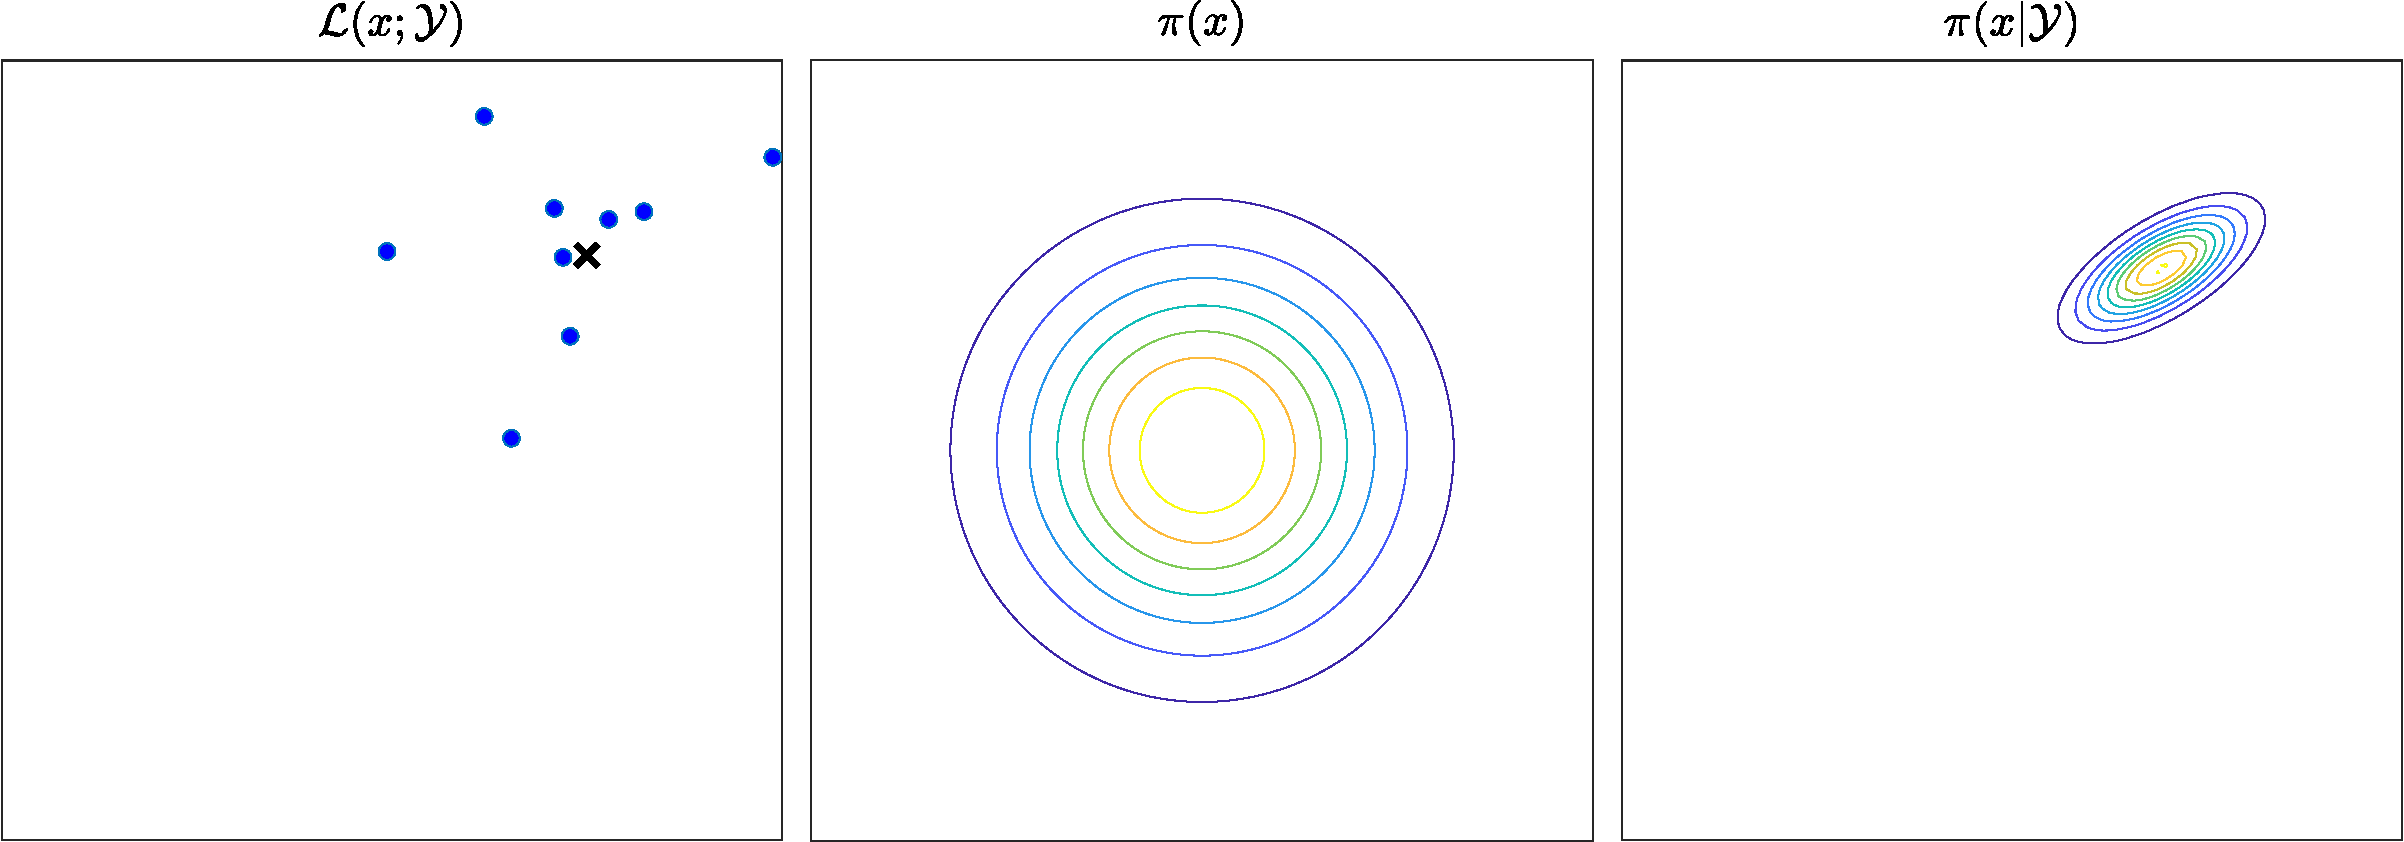
\includegraphics[width = 140mm]{Figures/figure-BI_2D.pdf}
    \caption{Bayesian inference in 2D space}
    \label{fig: BI_2D}
\end{figure}
\section{Posterior quantities of interest}
Under the Bayesian paradigm, the posterior distribution $\pi(\boldsymbol{x}|\mathcal{Y})$ is the solution of the inverse problem. However, in practice it can also serve as an intermediate result that is further processed for interpretation or prediction purpose. Furthermore, the full distribution can contain too much information to allow statements about the inferred parameters. Therefore, it is common to process the posterior and extract certain quantities of interest that summarize the inversion results more concisely.

In many applications, one is only interested in a single parameter, i.e., the one that characterise the inversion most suitably. The two most common \textit{point estimation} methods are the \textit{posterior mean} $\boldsymbol{x}^{\rm{mean}}$ and \acrfull{MAP}. The $\boldsymbol{x}^{\rm{mean}}$ is given as:
\begin{equation}
    \label{eq: posterior mean}
    x^{\rm{mean}} = \mathbb{E}[\boldsymbol{X}|\mathcal{Y}] = \int_{\mathcal{D}_{\boldsymbol{X}|\mathcal{Y}}} 
    \boldsymbol{x} \pi(\boldsymbol{x}|\mathcal{Y}) {\rm{d}} \boldsymbol{x}  
\end{equation}
It reflects what we expect the parameter value to be after the inference. The \acrshort{MAP} parameter, as the mode of the posterior distribution on the other hand, is the one maximises the posterior:
\begin{equation}
    \label{eq: MAP}
    \begin{aligned}
       \boldsymbol{x}^{\rm{MAP}} &= \mathop{\arg\max}\limits_{\boldsymbol{x} \in \mathcal{D}_{\boldsymbol{X}}}
    \pi(\boldsymbol{x}|\mathcal{Y}) \\
    &=\mathop{\arg\max}\limits_{\boldsymbol{x} \in \mathcal{D}_{\boldsymbol{X}}}
   {\mathcal{L}(\boldsymbol{x};\mathcal{Y}) \pi(\boldsymbol{x})}     
    \end{aligned}
\end{equation}
where the evidence constant $\pi(\mathcal{Y})$ was omitted. The \acrshort{MAP} point corresponds to the most likely value of the input parameters. It is closely related to the \acrfull{ML} point that is defined as 
\begin{equation}
    \label{eq: MLE}
    \boldsymbol{x}^{\rm{ML}}  = \mathop{\arg\max}\limits_{\boldsymbol{x} \in \mathcal{D}_{\boldsymbol{X}}}
   {\mathcal{L}(\boldsymbol{x};\mathcal{Y})}
\end{equation}
for which the forward model $\mathcal{M}$ produces the best agreement with the available data. Unlike the \acrshort{ML}, the \acrshort{MAP} point considers the prior information imposed by the prior distribution. The difference is typically larger in the case of little data, where the regularisation effect of the prior distribution is stronger. In case of uniform priors, the two are equal, provided that the \acrshort{ML} point does not lie outside the prior support.

Choices for the point estimation above disregards the estimation uncertainty in the parameters. Therefore, to more comprehensively characterise the posterior distribution and investigate the calibration, it is useful to compute the second $\textit{posterior moments}$ and the $\textit{covariance}$. They are summarised in the $\textit{posterior covariance matrix}$ $\boldsymbol{C} \in \mathbb{R}^{M \times M}$ with entries:
\begin{equation}
    \label{eq: COV}
    \begin{aligned}
    \boldsymbol{C}  &= {\rm{Cov}}[\boldsymbol{X}|\mathcal{Y}] \\
            &=\int_{\mathcal{D}_{\boldsymbol{X}}} 
            (\boldsymbol{x} - \mathbb{E}[\boldsymbol{X}|\mathcal{Y}])(\boldsymbol{x} - \mathbb{E}[\boldsymbol{X}|\mathcal{Y}])^{\mathsf{T}} \pi(\boldsymbol{x}|\mathcal{Y}) {\rm{d}} \boldsymbol{x} 
    \end{aligned}  
\end{equation}
\begin{figure}[htbp]
    \centering
    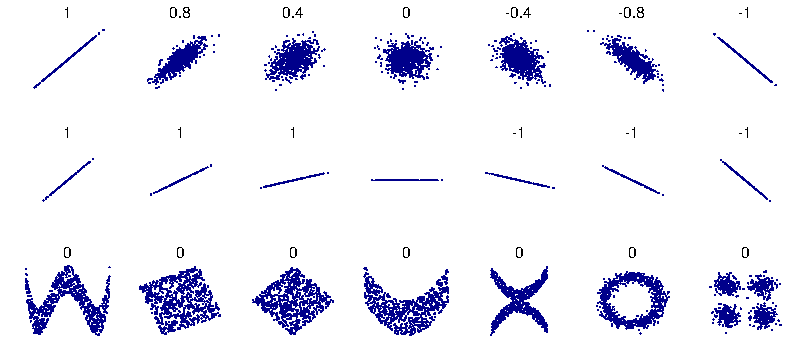
\includegraphics[width = 140mm]{Figures/figure-COV.pdf}
    \caption{Example sets of ($x,y$) points with different COV. Source: $\href{https://commons.wikimedia.org/wiki/File:Correlation_examples2.svg?uselang=zh-cn}{Wikipedia}$}
    \label{fig: COV}
\end{figure}
As  the full posterior distribution is an \textit{M}-dimensional object, which is inherently difficult to comprehend, one is typically also interested in the \textit{posterior marginals}. The distribution of the marginalised random variable $X_{i}|\mathcal{Y}$ is given by (see \cref{eq: Margin_Post}):
\begin{equation}
    \label{eq: Margin_Post}
    \pi(x_{i}|\mathcal{Y}) = \int_{\mathcal{D}_{\boldsymbol{X}_{\rm{\boldsymbol{v}}}}}
          \pi(\boldsymbol{x}|\mathcal{Y}){\rm{d}} \boldsymbol{x_{\rm{\boldsymbol{v}}}}, {\rm{with}} \ \boldsymbol{\mathrm{v}} = \{1,\cdots,M\} \backslash i  
\end{equation}
This univariate \acrshort{PDF} can be integrated to obtain the corresponding \acrfull{CDF} which may then be used to define \acrfull{CI} on the calibrated parameters by means of quantiles.

To assess the predictive capabilities of a computational model, the Bayesian inference framework offers the possibility to compute \textit{predictive distributions}. Using previously defined discrepancy model from \cref{eq: Gaussian discrepancy} and \cref{eq: discrepancy term}, the \textit{prior predictive} distribution can be written as:
\begin{equation}
    \label{eq: prior predictive}
    \pi(\boldsymbol{y}) = \int_{\mathcal{D}_{\boldsymbol{X}}} 
    \pi(\boldsymbol{x}) \pi(\boldsymbol{y}|\boldsymbol{x}) {\rm{d}} \boldsymbol{x}
\end{equation}
It summarises the uncertainty about the model output considering also the discrepancy model before calibration. It should in practice be used to determine whether the measured data can be reproduced and consequently rule out severely ill-posed inverse problems that should be re-evaluated before proceeding with expensive calibration procedures. The \textit{posterior predictive} distribution (see \cref{eq: posterior predictive}) can be similarly written as:
\begin{equation}
    \label{eq: posterior predictive}
    \pi(\boldsymbol{y}|\mathcal{Y}) = \int_{\mathcal{D}_{\boldsymbol{X}|\mathcal{Y}}} 
    \pi(\boldsymbol{x}|\mathcal{Y}) \pi(\boldsymbol{y}|\boldsymbol{x}) {\rm{d}} \boldsymbol{x}
\end{equation}
\section{Computational methods for Bayesian inference}
The practical computation of posterior distributions $\pi(\boldsymbol{x}|\mathcal{Y})$ is not trivial. Because computing evidence $\pi(\mathcal{Y})$ is usually not a tractable problem, analytical solutions thus require more restrictions on the model. It can be only calculated analytically if it is given in a closed form. A common strategy we usually choose is a \textit{conjugate prior} \citep{gelman1995} to the likelihood, so the integral can be represented analytically. For example, in a static Bayesian network, choices such as \textit{Variant elimination} and \textit{Belief propagation} \citep{murphy2012} can be seen. In the realm of a dynamic sequential model, \textit{kalman filtering} \citep{nguyen2016} gives an closed form for the parameter identification. However, in the general cases, the solution to the posterior can be rarely analytical due to a complex model or high computation for the evidence $\pi(\mathcal{Y})$. Thus, we need to resort to approximation method.

There are usually two categories of approximation methods: \textit{optimisation based approximation} and \textit{Monte Carlo sampling} methods.
\begin{itemize}[left=0pt]
    \item \textcolor{blue}{\textit{Optimisation based approximation}}: This method usually refers to variational inference. The basic idea of optimized based approximation is to use an analytical form of a distribution to approximate the posterior based on some loss functions. Then we can see the similarity (e.g., \textit{Kullback-Leibler divergence}) to measure in information contained within two distributions.
    
    The advantages of optimised approximation methods are: (1) Computationally efficient and work well on large models. (2) It has absolute converging criteria which makes easy to determine when to stop the modelling. (3) It scales better and are more amenable to parallelization. However, there are some problems itself: (1) Unlike \textit{sampling-based methods}, variational approaches will almost never find the globally optimal solution. (2) their accuracy is often limited by the form of the approximation.
    \item \textcolor{blue}{\textit{Monte Carlo sampling}}: Sampling method is another way to approximate the posterior distribution. Examples include \textit{inverse probability transform}, \textit{rejection sampling}, \textit{importance sampling}, \acrfull{MCMC} and \acrfull{SMC}. These methods generate random samples from a \textit{proposal distribution} and use them to estimate the posterior distribution and the derived statics.

    \textit{Monte Carlo sampling} has the advantages that: (1) It is more straightforward and flexible. (2) It is guaranteed to find the globally optimal solution given enough time and samples. However, In order to quickly reach a good solution, \textit{Monte Carlo sampling} take more time and require choosing an appropriate sampling technique. 
\end{itemize}

\textit{Optimisation based approximation} and \textit{Monte Carlo sampling} are a big topic. Current studies on these are still very active with numerous techniques proposed in the past few years. More discussions can be found in \cite{murphy2012} and \cite{blei2017}. 

\textit{Monte Carlo sampling} is asymptotically exact; \textit{Optimisation based approximation} is not. In the limit, \textit{Monte Carlo sampling} will exactly approximate the target distribution. \textit{Optimisation based approximation} comes without warranty.

In this thesis, however, we expect to find the global optimal values and hope the solution with guarantee. Therefore, our primary is only focused on \textit{Monte Carlo sampling}. 


\section{Approximation inference}

\subsection{Expectation maximization algorithm}

\subsection{Ensemble Kalman filter}
\subsection{Sequential Monte Carlo}
\begin{figure}[htbp]
    \centering
    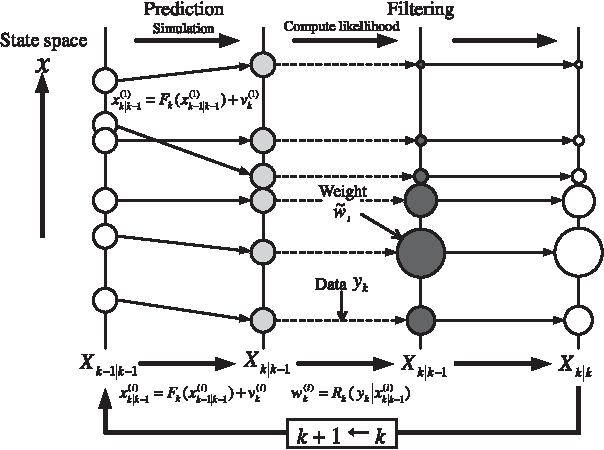
\includegraphics[width = 140mm]{Figures/figure-particle filter.pdf}
    \caption{Bayesian inference in 2D space}
    \label{fig: particle filter}
\end{figure}

\subsection{Markov Chain Monte Carlo}
\begin{figure}[htbp]
    \centering
    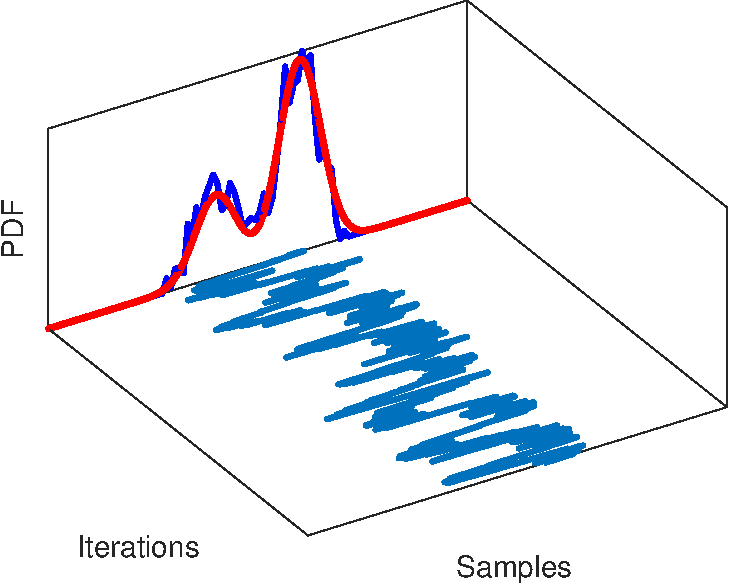
\includegraphics[width = 90mm]{Figures/figure-MCMC_sampling.pdf}
    \caption{\acrshort{MCMC} sampling}
    \label{fig: MCMC_sample}
\end{figure}



\chapter{Uncertainty quantification in high dimensions}
\label{UQ}

Uncertainty quantification (UQ) endeavors to consider the uncertainties associated with the parameters in the model of a physical system and examine their influence on the system response. A well-established representation of an uncertainty quantification problem is outlined next. The premise is that any such problem can be depicted as a combination of these ingredients, as illustrated in \cref{fig: UQ_steps}:
\begin{itemize}
    \item A computational model $\mathcal{M}$. This encompasses a broad spectrum, ranging from an analytical function in its simplest form to a black box housing various levels of partial differential equations (e.g., finite element packages or finite difference packages). Generally, the computational model $\mathcal{M}$ establishes a mapping from a set of input parameters $\boldsymbol{x})$ to one or more \acrfull{QoI}, often denoted as \textit{model responses}.    
    \item The sources of uncertainties in input space. This step involves identifying the input parameters that are uncertain and describing them within a probabilistic context.
    \item Uncertainty propagation from input parameters $\boldsymbol{x}$ to $\boldsymbol{y}$. This step pertains to quantifying the \acrshort{QoI} by propagating the uncertainty of the input space through the computational model $\mathcal{M}$. 
    \item Iterative updating of the source of uncertainty. This step encompasses various techniques employed to refine the information related to the identified sources of uncertainty above. Examples includes \textit{sensitivity analysis} or \textit{Bayesian inference}. If we are using \textit{sensitivity analysis} to update the uncertainties, it can be explicitly called as \textit{forward problems}. If we are using \textit{Bayesian inference} to update the uncertainties, it can be called as \textit{inverse problems}.
\end{itemize}
\begin{figure}[htbp]
    \centering
    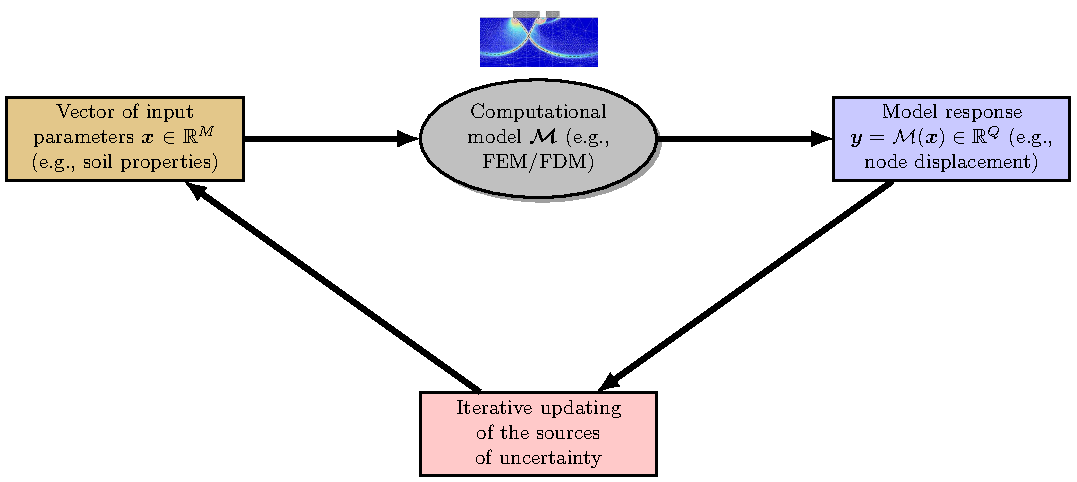
\includegraphics[width = 140mm]{Figures/figure-UQ_steps.pdf}
    \caption{Global framework for uncertainty quantification}
    \label{fig: UQ_steps}
\end{figure}


\section{Challenges}
In modern engineering applications, uncertainty quantification (UQ) often involves simulations with a large number of input parameters. The computational model is frequently treated as a black box, where only the input parameters $\boldsymbol{x}$ and the corresponding model response $\boldsymbol{y}$ are available. Addressing uncertainties through traditional \textit{Monte Carlo} methods in such systems can be computationally intensive, posing a significant challenge. To alleviate this computational burden, surrogate models $\tilde{\mathcal{M}}$, illustrated in \cref{fig: UQ_surrogate}, can be employed. The solid line denotes the current working flow. These surrogate models approximate the original model with a cost-effective replacement model, allowing for efficient exploration of the input parameter space. 
\begin{figure}[htbp]
    \centering
    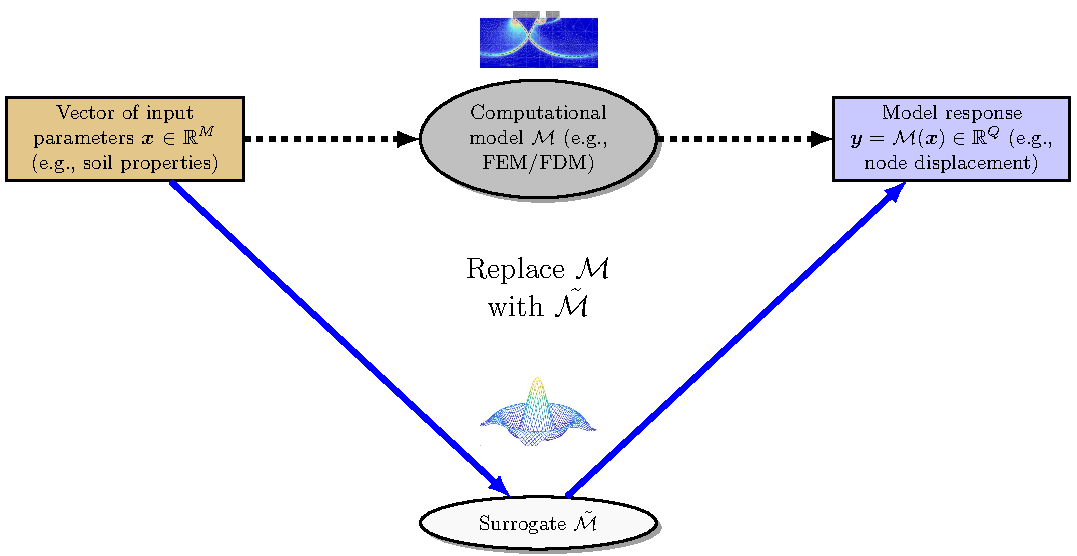
\includegraphics[width = 140mm]{Figures/figure-UQ_surrogate.pdf}
    \caption{Using a surrogate to obtain the model response}
    \label{fig: UQ_surrogate}
\end{figure}

 In high dimensions scenarios, surrogate models tend to exhibit diminished performance, coupled with escalating computational and storage costs-a challenge commonly acknowledged as the \textit{curse of dimensionality}. Consequently, challenges may arise from: 
 (1) in large-scale scenarios, the computational intractability of conducting thousands of forward simulations is a common challenge; (2) the complexity of the input/output space dimensions adds another layer of difficulty;(3) the large dimensionality of the input/output space complicates the sampling process;
 Thus, to alleviate this in a statistical inverse problems, methods can be broadly categorized in three groups: (1) choose an appropriate type of surrogates to accelerate a forward simulation; (2) reduce the size of the input/output space, i.e., sensitive analysis or \acrlong{DR} techniques; (3) sequential efficient sampling method in \textit{experiment of design} (\textit{active learning}) or in a posterior (e.g., \acrshort{MCMC}).


\section{Surrogate model choices}
 

\begin{table}[htbp]
\caption{Surrogate model choices}
\label{table: All_Surrogates}
\begin{tabular}{lll}
\hline
Name                              & \multicolumn{1}{c}{Shape} & \multicolumn{1}{c}{Parameters} \\ \hline
Polynomial chaos expansions       &                           $\tilde{\mathcal{M}}(\boldsymbol{x})
=
\sum_{\boldsymbol{\alpha} \in \mathcal{A} } 
\boldsymbol{y_{\alpha}} \Psi_{\boldsymbol{\alpha}} (\boldsymbol{x})$&                                $\boldsymbol{y_{\alpha}}$\\
Low-rank tensor approximations    &                           $\tilde{\mathcal{M}}(\boldsymbol{x})
=
\sum_{l=1}^{R} b_{l}
\left ( 
\prod_{i=1}^{M}  v_{l}^{i}x_{i}
 \right ) 
$&                                $b_{l}, \  z_{k,l}^{i}$\\
Kriging (a.k.a Gaussian processs) &                           $\tilde{\mathcal{M}}(\boldsymbol{x})
=
\boldsymbol{\beta}^{T} \cdot \boldsymbol{f}(\boldsymbol{x})
 + Z(\boldsymbol{x},\omega)$&                                $\boldsymbol{\beta}, \ \sigma_{Z}^{2}, \  \boldsymbol{\theta}$\\
Support vector machines           &                           $\tilde{\mathcal{M}}(\boldsymbol{x})
=
\sum_{i=1}^{m}
a_{i} K(\boldsymbol{x}_{i},\boldsymbol{x}) 
+b$&                                $\boldsymbol{a}, \ b$\\
Neural networks                   &                           $\tilde{\mathcal{M}}(\boldsymbol{x})
=
f_{n}\left ( 
\cdots f_{2}(
b_{2} + f_{1}(
b_{1} + \boldsymbol{w}_{1} \cdot \boldsymbol{x}
)
\cdot \boldsymbol{w}_{2}
)
\right ) $&                                $\boldsymbol{w}, \ \boldsymbol{b}$\\ \hline
\end{tabular}
\end{table}
Ongoing research on surrogate modelling focuses on various problems, like hyperparametes tuning, mathematical explanation or the accuracy based on few observations \citep{torre2019}. A range of techniques exist in surrogate modelling, in which some of them are listed in the \cref{table: All_Surrogates}. Among these popular surrogate models above, it is crucial to choose the most appropriate model for our own geotechnical problem. Inspired by \cite{torre2019}, we only focus on \acrfull{PCE}. Compared with other surrogate models based on benchmark data sets (e.g., \textit{Ishigami function}, \textit{23-bar horizontal truss}), \acrshort{PCE} exhibits:
\begin{itemize}[left=0pt]
    \item \acrshort{PCE} excels in various tasks, necessitating only minimal parameters tuning for adaptation to specified data considerations.
    \item \acrshort{PCE} not only provides precise point-wise predictions for the output at given inputs, but also furnishes relevant statistics in the presence of input uncertainties. This benefits in UQ process as it results from the integration of the \acrshort{PCE} model with a suitable probabilistic characterisation of the input model.
    \item The coefficients of \acrshort{PCE} can readily be transformed to output sensitivity analysis results.
    \item The output produced by \acrshort{PCE} is analytically expressed as a simple polynomial of the input. This characteristic makes the model easy to interpret from a mathematical standpoint. This is in contrast with black-box models (e.g., neural networks) or classification-based models (e.g., tree models), where our reliance is placed on the assumption that training data is sufficiently big to yield an accurate surrogate.
    \item \acrshort{PCE} achieves acceptable performance levels with a relatively 
    modest amount of data in the \textit{experiment of design}.
\end{itemize}
Note: The choice for \acrshort{PCE} in our thesis does not guarantee the conclusion that \acrshort{PCE} outperforms than other surrogate models. The properties obtained above are only based on some simple toy problems. Therefore, a choice for surrogate models is problem-specified and it is not always the same case when it encounters into different geotechnical problems.


\section{Polynomial chaos expansion}
Polynomial chaos expansions (PCE) represent a potent surrogate modelling technique designed to provide a functional approximation of a computational model. This approximation is achieved through its spectral representation of the model on a carefully built basis of polynomial functions. Consider a random vector with independent components $\boldsymbol{X} \in \mathbb{R}^{M}$ characterized by the joint \acrshort{PDF} $f_{\boldsymbol{X}}$. Additionally, suppose there exists a computation model with finite variance, defined as a mapping $Y = \mathcal{M}(\boldsymbol{X})$, with $Y \in \mathbb{R}$. This can be expressed as follows:
\begin{equation}
    \mathbb{E}[Y^2] 
    =\int_{\mathcal{D}_{\boldsymbol{X}}}
    \mathcal{M}^2(\boldsymbol{x})f_{\boldsymbol{X}}(\boldsymbol{x})
    d\boldsymbol{x}< \infty 
\end{equation}
Then, a \acrshort{PCE} $\mathcal{M}(\boldsymbol{X})$ can be represented as:
\begin{equation}
\label{eq: PCE_basis}
Y=\mathcal{M}(\boldsymbol{X}) \approx
\sum\limits_{\alpha \in \mathcal{A} }{\boldsymbol{y_{\alpha}} \Psi_{\boldsymbol{\alpha}}(\boldsymbol{X})}
\end{equation}
where $\Psi_{\boldsymbol{\alpha}}(\boldsymbol{X})$ denotes multivariate polynomials orthonormal relative to $f_{\boldsymbol{X}}$, The multi-index $\boldsymbol{\alpha} \in \mathcal{A}$ identifies the truncated multivariate polynomials $\Psi_{\boldsymbol{\alpha}}$. $\boldsymbol{y_{\alpha}} \in \mathbb{R}$ corresponds to the corresponding coefficients. There are four main ingredients for a \acrshort{PCE}: (1) Construct the basis functions $\Psi_{\boldsymbol{\alpha}}$; (2) Compute the coefficients $\boldsymbol{y_{\alpha}}$; (3) Evaluate the precision of the \acrshort{PCE}; (4) Post process the \acrshort{PCE}. A visualized \acrshort{PCE} example with a two-dimensional input can be seen in \cref{fig: PCE_visual}.
\begin{figure}[htbp]
    \centering
    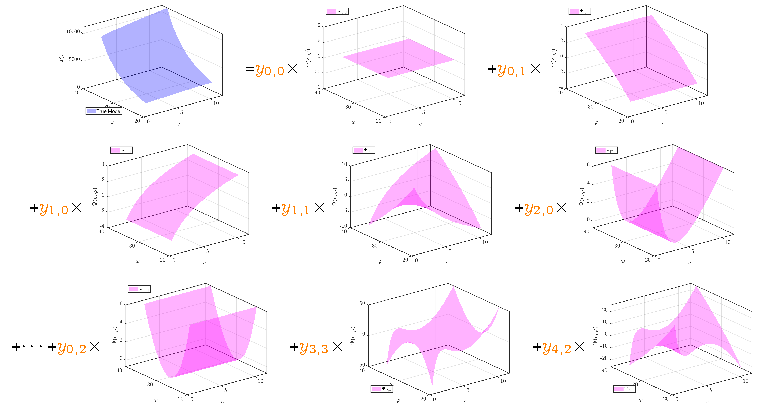
\includegraphics[width = 140mm]{Figures/figure-PCE_visualize.pdf}
    \caption{PCE visualization in a two-dimensional example from \protect\cite{PCE-visual}}
    \label{fig: PCE_visual}
\end{figure}



\subsection{Construct the basis functions $\Psi_{\alpha}$}
The polynomial basis $\Psi_{\boldsymbol{\alpha}}(\boldsymbol{x})$ in \cref{eq: PCE_basis} is conventionally constructed using a set of \textit{univariate orthonormal polynomials} $\phi_{k}^{i}(x_{i})$, where these polynomials satisfy:
\begin{equation}
    \left \langle 
\phi_{j}^{i},\phi_{k}^{i}
 \right \rangle 
= \delta_{jk}
\end{equation}
$\delta_{jk}$ is the \textit{Kronecker symbol}. The multivariate polynomials $\Psi_{\alpha}$ are then constructed by taking the tensor product of their univariate counterparts:
\begin{equation}
\Psi_{\boldsymbol{\alpha}}(\boldsymbol{x})
 \overset{\mathrm{def}}{=}
\prod_{i=1}^{M} 
\phi_{\alpha_{i}}^{i}(x_{i})
\end{equation}
in which, $\boldsymbol{\alpha}= \{\alpha_{1},\cdots,\alpha_{M}\}  \ \alpha_{i} \in \mathbb{N}^{M}$ of degree $|\boldsymbol{\alpha }|=\sum_{i=1}^{M} \alpha_{i}$, and $\Psi_{\boldsymbol{\alpha}}(\boldsymbol{x})$ satisfies orthonormal properties as:
$        \left \langle 
\Psi_{\boldsymbol{\alpha}}(\boldsymbol{x}),\Psi_{\boldsymbol{\beta}}(\boldsymbol{x})
 \right \rangle 
= \delta_{\boldsymbol{\alpha}\boldsymbol{\beta}}$, where the symbol $\delta_{\boldsymbol{\alpha}\boldsymbol{\beta}}$ is an extension \textit{Kronecker symbol} to the multi-dimensional case. Classical families of orthogonal polynomials have been discovered historically in \cref{table: Polynomial_family}. 
\begin{table}[]
\caption{Univariate orthogonal polynomials}
\label{table: Polynomial_family}
\centering
\begin{tabular}{lll}
\hline
\textbf{Name}& \textbf{Support $\mathcal{D}_{\boldsymbol{X}}$}& \textbf{Weight function $f_{\boldsymbol{X}}$}\\ \hline
Legendre&            $[a;b]$&                    uniform\\
Jacobi&            $[a;b]$&                    Beta\\
Hermite&            ($-\infty;\infty$)&                    Gaussian\\
Laguerre&            $[;\infty)$&                    Gamma\\ \hline
\end{tabular}
\end{table}
\begin{equation}
A^{M,p,q} = \{\alpha \in A^{M,p} : ||\alpha||_q \leq p\}; \ {\rm{where}}  \   
||\alpha||_q = \left(\sum_{i=1}^{M} \alpha_i^q\right)^{1/q}
\end{equation}
The infinite series expansion cannot be handled in practical computations. Two truncation schemes can be applied: (1) restriction of maximum interaction $p$; (2) reduce hyperbolic truncation $q$. An example of the truncation in two dimensions for various values of $p$ and $q$ is depicted in \cref{fig: PCE_truncation}.
\begin{figure}[htbp]
    \centering
    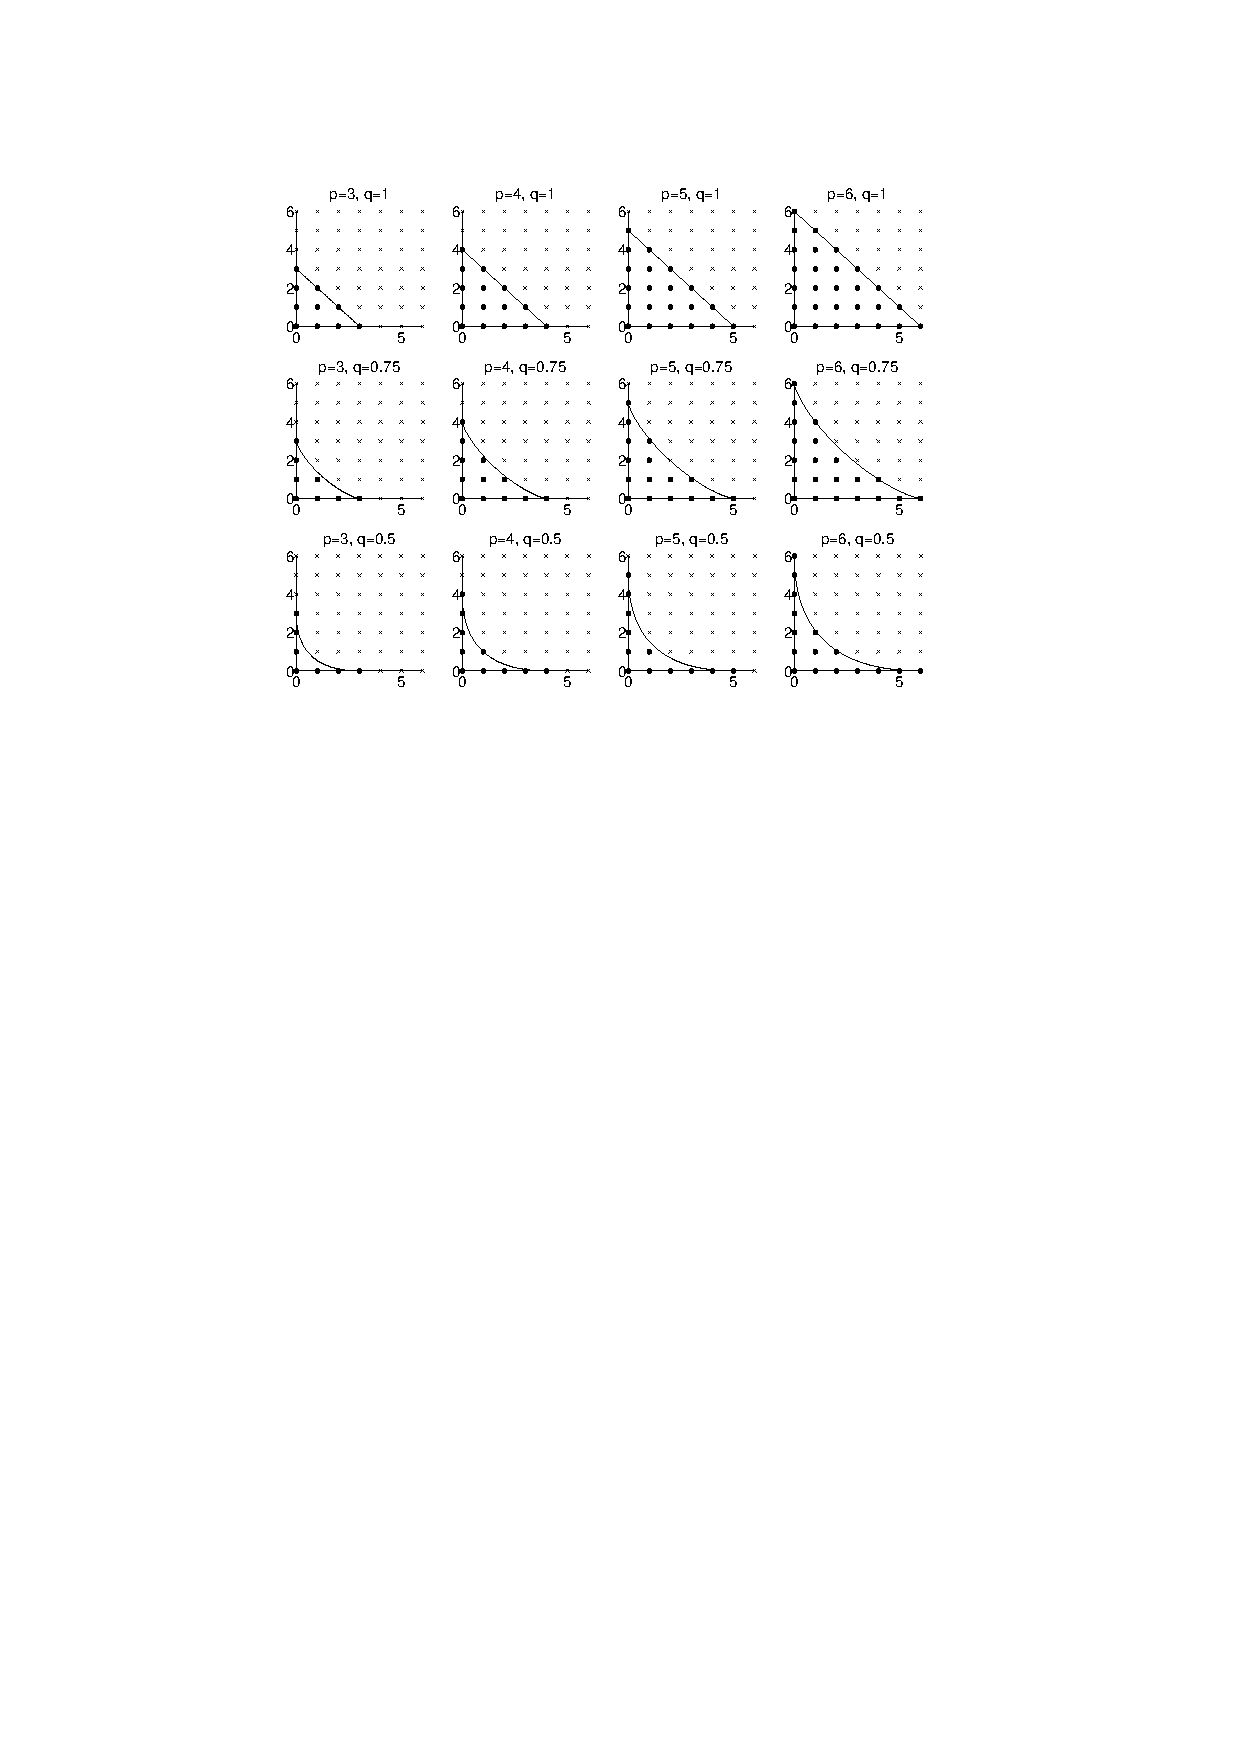
\includegraphics[width = 140mm]{Figures/figure-PCE_truncation.pdf}
    \caption{Truncation set for varying values of $p$ and $q$ from \cite{UQdoc}}
    \label{fig: PCE_truncation}
\end{figure}


\subsection{Compute the coefficients $y_{\alpha}$}
Various methods are available for computing the coefficients $\boldsymbol{y_{\alpha}}$ of the \acrshort{PCE} with a known basis. Two primary strategies commonly employed are \textit{projection} and \textit{regression}. \textit{Projection} methods leverage the orthogonality of the basis to determine the coefficients. On the other hand, \textit{regression} methods utilize standard linear regression approaches to solve the system. Below are some of the methods:

\subsubsection{Projection method}
The evaluation of the polynomial coefficients $\boldsymbol{y_{\alpha}}$ can be reformulated as the calculation of the expectation value in 
\begin{equation}
\label{eq: PCE_projection}
\boldsymbol{y_{\alpha}} = E [\Psi_{\boldsymbol{\alpha}}(\boldsymbol{X}) \cdot \mathcal{M}(\boldsymbol{X})]
\end{equation}

\subsubsection{Least-squares minimization}
This approach casts \cref{eq: PCE_projection} as a least-squares minimisation problem as shown:
\begin{equation}
\boldsymbol{\hat{y}_{\alpha}} = {\rm{argmin}} \mathbb{E} [\varepsilon_{P}^2(\boldsymbol{X})] = {\rm{argmin}} \mathbb{E} [(\tilde{\mathcal{M}}(\boldsymbol{X}) - \mathcal{M}(\boldsymbol{X}))^2]
\end{equation}
Some other regression methods can be also implemented, i.e., \textit{ordinary least square}, \textit{compressive sensing} or \textit{stochastic collocation}.


\subsection{Accuracy of the \acrshort{PCE}}
Error estimators are essential for quantifying the fidelity of a surrogate model in approximating the original model. To determine the precision of a surrogate, \textit{leve-one-out} (LOO) is a good way to assess the cross validation error. For a \acrshort{PCE} consisting $N$ metamodels, error $\varepsilon_{\text{LOO}}$ can be shown as:
\begin{equation}
\varepsilon_{\text{LOO}} = \frac{1}{N} \sum_{i=1}^{N} \left( \mathcal{M}(\boldsymbol{x}^{(i)}) - \tilde{\mathcal{M}}(\boldsymbol{x}^{(i)}) \right)^2
\end{equation}




\subsection{Post process the \acrshort{PCE}}
Due to the inherent orthogonality with the polynomial basis functions, we can derive explicit expressions for moments characterizing the model output. The first pair moments of a \acrshort{PCE} find their manifestation within is coefficients. Specifically, the mean and variance of a \acrshort{PCE} manifest as:
\begin{equation}
E[Y] = \mathbb{E}[\tilde{\mathcal{M}}(\boldsymbol{X})] = y_{\boldsymbol{0}}
\end{equation}
\begin{equation}
\text{Var}[Y] = E[Y^2] - E[Y]^2  \approx \sum_{\alpha \in A \setminus \{0\}} y_{\alpha}^2
\end{equation}
Another crucial aspect of \acrshort{PCE} post-processing lies in the fact the coefficients encapsulate significant details regarding the \textit{ANOVA} decomposition of a surrogate. This information can be harnessed to efficiently compute global sensitivity at a minimal computational expense. 

\section{Dimensionality reduction}


Geotechnical problems inherently involve high dimensionality, posing challenges for learning methods like surrogate modeling. Technical constraints impact the storage and processing of such large amounts of data. Furthermore, as input and output data expand, independent scalar surrogate models show inadequate in accurately capturing the covariance matrix of the original data, leading to less reliable predictions. Consequently, in high dimensional space, \acrfull{DR} is critical. 

The transformation from the \textit{original space} $\mathcal{D}_{\boldsymbol{Y}} \subseteq \mathbb{R}^{N}$ to a \textit{reduced space} $\mathcal{D}_{\boldsymbol{Z}} \subseteq \mathbb{R}^{n}$ with $n \ll N$ is the general form of a \acrshort{DR} mapping:
\begin{equation}
    \mathcal{T}_{DR} : \mathcal{D}_{\boldsymbol{Y}} \rightarrow \mathcal{D}_{\boldsymbol{Z}}
\end{equation}
where the underlying assumption is that $\mathcal{D}_{\boldsymbol{Z}}$ is embedded inside $\mathcal{D}_{\boldsymbol{Y}}$. There exists a large set of \acrshort{DR} techniques ranging from linear to nonlinear approaches. A simple but effective linear technique, that is widely used today, is the \textit{principal component analysis} (\acrshort{PCA}). It is popular across a wide range of disciplines and is closely related to the \textit{Karhunen-Loève expansion} and \textit{proper orthogonal decomposition}. In practical applications, the \acrshort{PCA} process is involves the estimation of the expectation $\boldsymbol{\mu_{Y}} \approx \mathbb{E}[\boldsymbol{Y}]$ and the covariance matrix $\Sigma_{\boldsymbol{Y}} \approx Cov[\boldsymbol{Y}]$. The $N$ eigenvectors of this covariance matrix are represented by $\phi_{p}$ for $p=1,\cdots,N$. The corresponding eigenvalue $\lambda_{p}$ signifies the variance of $\boldsymbol{Y}$ in direction of the $p-th$ principle component. Consequently, the random vector $\boldsymbol{Y}$ can be expressed through its $n$ principal components with the highest variance:
\begin{equation}
\boldsymbol{Y} \approx \boldsymbol{Y}^{PCA} 
= \boldsymbol{\mu_{Y}} + 
\sum_{p=1}^{n} z_{p}\phi_{p}
\end{equation}
The selection of the number $n$ is determined such that $\sum_{p=1}^{n} \lambda_{p} = 
(1-\varepsilon_{0})\sum_{p=1}^{N} \lambda_{p}$, where $\varepsilon_{0}$ typically set to 0.01. Consequently, the model output $\boldsymbol{Y} \in \mathbb{R}^{N}$ can be processed by a linear transformation of the principle component vector $\boldsymbol{Z} = (z_{1},\cdots,z_{n})$. This reduction in the dimensionality, from $N$ to $n$ $n \ll N$, is then achieved. When data sets become more complex, more advanced \acrshort{DR} techniques can be used, such as \textit{multi-dimensional scaling}, \textit{kernel principal component analysis} and \textit{auto-encoder}.


\section{DR-based surrogate in Bayesian inference}
In high dimensions, a popular two-step approach is frequently adopted to address such challenges: first, the input/output dimensions are reduced; subsequently, the surrogate model is directly constructed within the \textit{reduced space}. Performance of DR-based surrogate has showed superior performance in some benchmarks \citep{lataniotis2019}. Take \acrshort{PCA} and \acrshort{PCE} as a \acrshort{DR} example in \cref{fig: PCA-PCE}, the amalgamation of \acrshort{PCA}-\acrshort{PCE} constitutes an efficient surrogate modelling technique. The solid line denotes the current working flow. 

\begin{figure}[htbp]
    \centering
    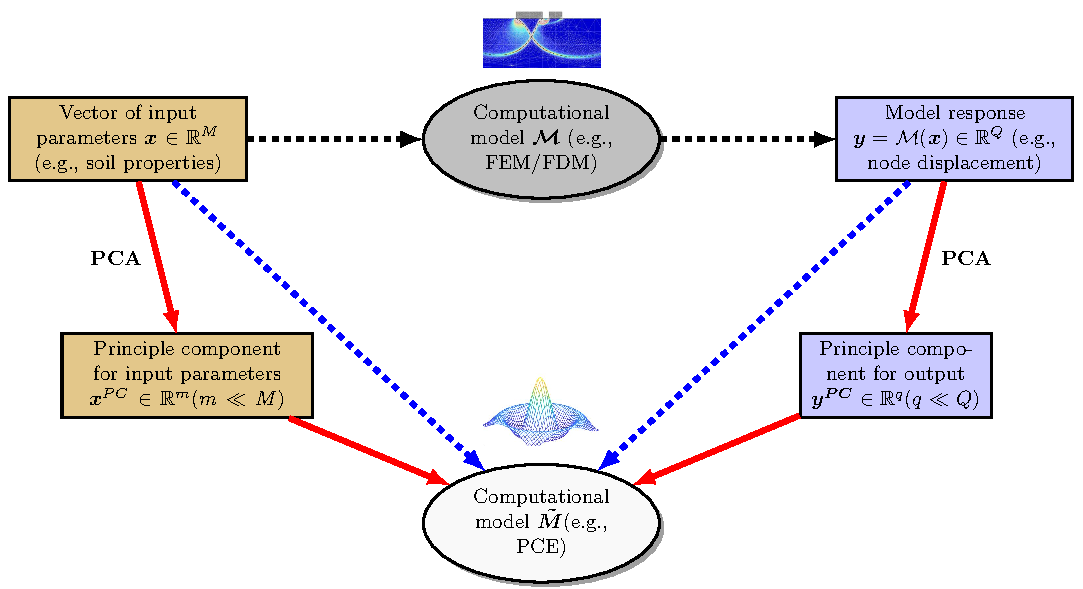
\includegraphics[width = 140mm]{Figures/figure-PCA_PCE.pdf}
    \caption{\acrfull{DR} schematic example}
    \label{fig: PCA-PCE}
\end{figure}
When it comes to Bayesian inference process accelerated by DR-based surrogate, working principles can be shown in \cref{fig: PCA-PCE-BI} as below:
\begin{itemize}[left = 0pt]
    \item Step one: \acrshort{PCA} technique reduces the size of input/output into principal components.
    \item Step two: construct \acrshort{PCE} based on the principal components from step one.
    \item Step three: Pass obtained \acrshort{PCE} into Bayesian inference process and evaluate the likelihood. 
\end{itemize}
\begin{figure}[H]
    \centering
    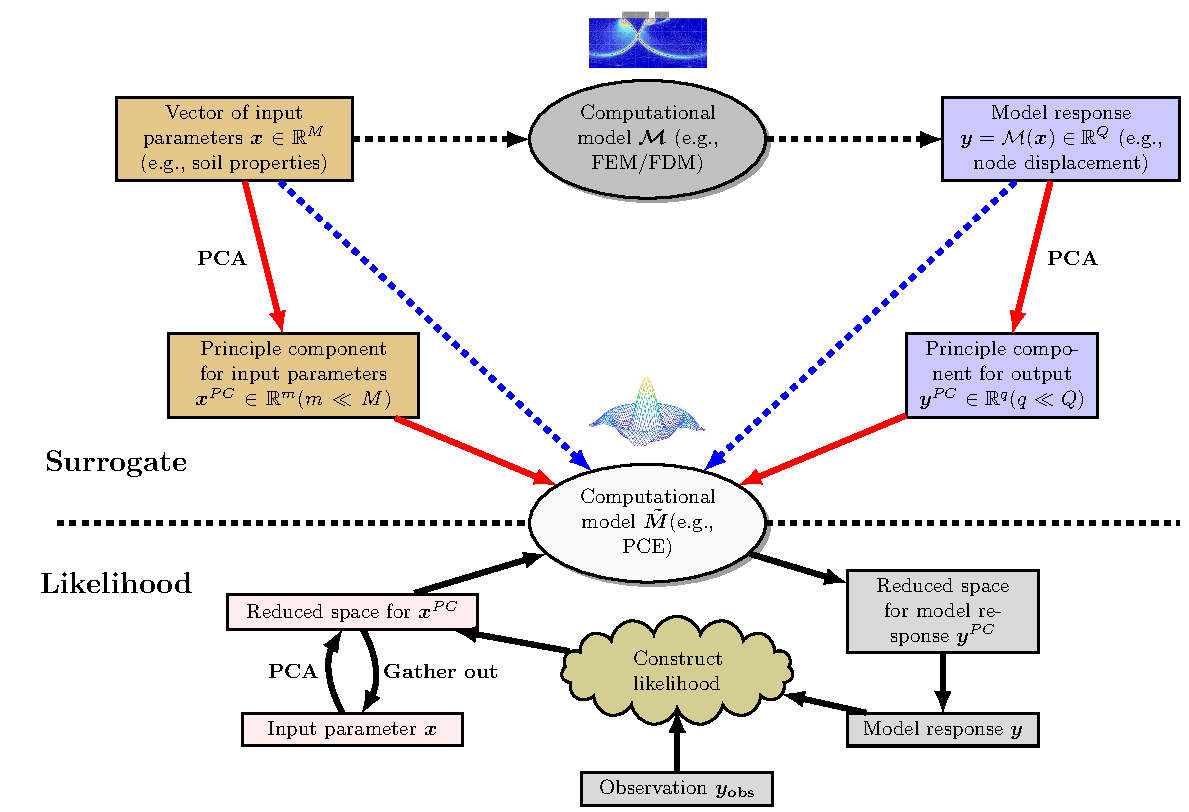
\includegraphics[width = 140mm]{Figures/figure-PCA_PCE_BI.pdf}
    \caption{Bayesian inference accelerated by a PCA-PCE surrogate}
    \label{fig: PCA-PCE-BI}
\end{figure}
It is worthy noting that DR-based surrogates are not only limited to Bayesian inference in high dimensions. Even in low dimension's inference, DR-based surrogates still outperform than the case with surrogate models without any \acrshort{DR}. Because \acrshort{DR} is more than a data compressing technique in Bayesian inference, it can capture the covariance matrix of the original data to make more accurate predictions. Due to this feature, compared to the traditional scalar models (e.g., PCE, kriging), DR-based surrogates make it possible to consider multiple outputs predictions.








\chapter{Predictive digital twins at scale for piles}
\label{DT}

This chapter develops a mathematical and computational foundation for digital twins of piles.

While the value proposition of digital twins has become widely appreciated, the technology itself remains in a custom production phase.



\section{State space model}




State space model, also called dynamic model, usually represents a class of directed probabilistic graphical model that describes the dependence between the hidden variables $\boldsymbol{Z} = (\boldsymbol{Z_0},\boldsymbol{Z_1},\boldsymbol{Z_2},...,\boldsymbol{Z_t})$ and the observed variables $\boldsymbol{X} = (\boldsymbol{X_1},\boldsymbol{X_2},...,\boldsymbol{X_t})$. This model also enables a dynamical updating for state estimation and control because they allow for recursive analysis of the systems in the time domain. As shown in \cref{fig: state-space-model}, this sequential updating feature is very suitable to geotechnical problems, because in our real life the observations typically appear in time series.



Based on the different assumptions for the model, state space model can be categorized as: Hidden Markov model, linear Gaussian state space model and Nonlinear non-Gaussian state space model.
\begin{figure}[H]
    \centering
    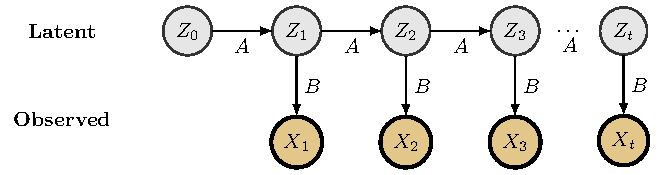
\includegraphics[width = 140mm]{Figures/figure-SSM.pdf}
    \caption{State space model}
    \label{fig: state-space-model}
\end{figure}
where gray circles $\boldsymbol{Z}$ are latent variable; bold outlines $\boldsymbol{X}$ are observed quantities; $A$ is the transition equation; $B$ is the observation equation. $A$ and $B$ are not time-varying.

\subsection{Hidden Markov model}

        
If the latent variables $\boldsymbol{Z} = (\boldsymbol{Z_0},\boldsymbol{Z_1},\boldsymbol{Z_2},...,\boldsymbol{Z_t})$ in \cref{fig:state-space-model} are discrete, we can treat the state space model as a hidden Markov model.  A hidden Markov model (HMM) allows us to talk about both observed events  $\boldsymbol{X}$ and hidden discrete events  $\boldsymbol{Z}$. A first-order hidden Markov model instantiates two simplifying assumptions as:

\begin{itemize}
      \item  First, as with a first-order Markov chain, the probability of a particular state depends
 only on the previous state:
         \begin{equation}
         P(Z_t|Z_0,Z_1,...,Z_{t-1})= P(Z_t|Z_{t-1})             
         \end{equation}      
      \item Second, the probability of an  observation $X_t$ depends only on the state that
 produced the observation $Z_t$ and not on any other states or any other observations:
          \begin{equation}
         P(Z_t|Z_0,Z_1,...,Z_{t-1})= P(Z_t|Z_{t-1})             
         \end{equation} 
\end{itemize}
In geotechnical area, filtering problem is more a quantity of interest. That is to say, given the current belief state $p(Z_{t-1}|X_{1:t-1})$, the primary concern next is how to calculate the belief state $p(Z_t|X_{1:t-1})$.
A prominent application for Hidden Markov model is addressing soil classification challenges with time series data. This is due to the discrete nature of the labeling predicament inherent in this context. However, the limitation for the HMM is also obvious. For the continuous state changing with time (e.g., soil stress, loading force or cumulative plastic strain), HMM is not suitable for such problem because infinite transition matrix $A$ does not exist. To solve this, we will discuss linear Gaussian model and nonlinear non-Gaussian model next. 







\subsection{Linear Gaussian state space model}

Linear Gaussian state space model is an exact Bayesian filtering solution, also called Kalman filter. Kalman filter describe a very specific setting, i.e., linear transition/observation equations and Gaussian noises. Since everything is Gaussian, we can perform the prediction and update steps in closed form,
 as we explain below:
% \setlength\abovedisplayskip{2pt}
% \setlength\belowdisplayskip{2pt}
\begin{equation}
\label{eq: Bayesian filtering}
\begin{aligned}
   & \boldsymbol{{z}_{t}}  =\boldsymbol{A} \boldsymbol{{z}_{t-1}}+\boldsymbol{w_{t}}  
  \ \ &\boldsymbol{w_{t}}   \sim \mathcal{N}\left(0, \boldsymbol{Q} \right) \\    
    &p(\boldsymbol{{z}_{t}}|\boldsymbol{{z}_{t-1}}) = \mathcal{N}(\boldsymbol{A} \boldsymbol{{z}_{t-1}},\boldsymbol{Q})    
    \\
     &\boldsymbol{{x}_{t}}=\boldsymbol{B} \boldsymbol{{z}_{t}}+\boldsymbol{v_{t}}  \ \ &\boldsymbol{v_{t}} \sim \mathcal{N}\left(0, \boldsymbol{R} \right)\\
     &p(\boldsymbol{{x}_{t}}|\boldsymbol{{z}_{t}}) = \mathcal{N}(\boldsymbol{B} \boldsymbol{{z}_{t}},\boldsymbol{R})   
\end{aligned}
\end{equation}
which stands for the prediction step and correction step, respectively.

The detailed principle of Kalman filter is not extensively emphasized here, because in geotechnical engineering, the transition and observation equations always show high nonlinearity. Once we add the SSM parameters to the state space model, the model is generally no longer linear Gaussian. Consequently
we must use some of the approximate online inference methods to be discussed below.

\subsection{Nonlinear non-Gaussian state space model}

Desipte the fact that some methods like Ensemble Kalman filter (EnKF), Unscented Kalman filter (UKF) or Extended kalman filter (EKF) can relax the linearity at some degree. These methods are still designed only for Gaussian posterior, which is not suitable for geotechnical problems with high nonlinearity. To handle the arbitrary posteriors, particle filtering which is based on Monte Carlo, can approximate the posterior with the increasing sampling points.



\section{Probabilistic graphical model: Control theory }




\section{Partially observable Markov decision process}

As shown in \cref{fig: POMDP}, based on Markov Chain, with introducing Rewards and Actions, it can form the basis of Partially observed Markov decision process.
\begin{figure}[H]
    \centering
    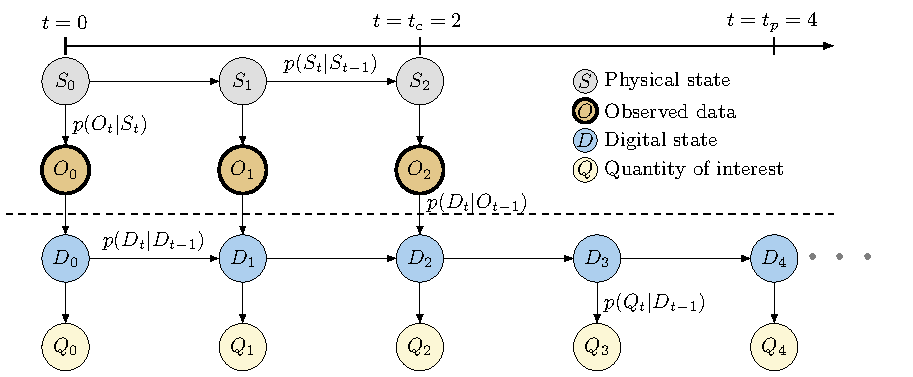
\includegraphics[width = 140mm]{Figures/figure-POMDP.pdf}
    \caption{Digital twin}
    \label{fig: POMDP}
\end{figure}
Generally, Digital Twin can be divided into two main parts, including (1) calibration and assimilation (2) Prediction, as shown in \cref{eq: DA_predict}  and \cref{eq: DA_assimilation}.
\begin{equation}
\begin{aligned}
& p(D_{0},...,D_{t_{c}},Q_{0},...,Q_{t_{c}},R_{0},...,R_{t_{c}}|o_{0},...,o_{t_{c}},u_{0},...,u_{t_{c}}) \\
& = \prod_{t=0}^{t_{c}}[\phi_{t}^{update}\phi_{t}^{QoI}\phi_{t}^{evaluation}] \label{eq: DA_predict}
\end{aligned}
\end{equation}
\begin{equation}
\begin{aligned}
    & p(D_{0},...,D_{t_{p}},Q_{0},...,Q_{t_{p}},R_{0},...,R_{t_{p}},U_{t_{c}+1},...,U_{t_{p}}|o_{0},...,o_{t_{c}},u_{0},...,u_{t_{c}}) \\
    & \propto \prod_{t=0}^{t_{p}}[\phi_{t}^{dynamics}\phi_{t}^{QoI}\phi_{t}^{evaluation}] \prod_{t=0}^{t_{c}}\phi_{t}^{assimilation} \prod_{t=t_{c}+1}^{t_{p}}\phi_{t}^{control} \label{eq: DA_assimilation}
\end{aligned}
\end{equation}
\section{Computational model-ICFEP}

\section{Planning and prediction via digital twin}
\chapter{Work Plan}

\label{Work_Plan}

\section{Stage 1}
Calibrate the models in \cref{fig:fig-CM2pile} with partially observed Markov decision process.
\begin{figure}[H]
    \centering

    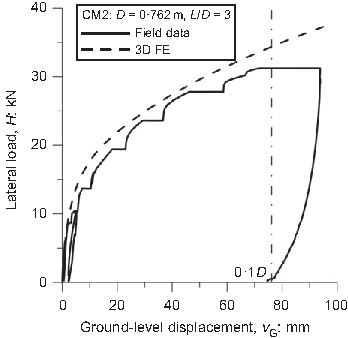
\includegraphics[width = 90mm]{Figures/figure-CM2.pdf}
    \caption{CM2 pile load displacement from \protect\cite{zdravkovic2020}}
    \label{fig:fig-CM2pile}
\end{figure}

\begin{itemize}
    \item Software: ICFEP-Likelihoods and observed data.
    \item Constitutive model: clay in \cite{zdravkovic2020} and sand in \cite{taborda2020}.
    \item Consider the soil profile variance-Create the random field (scale of fluctuation in ICFEP).
\end{itemize}
Objective: Ensure the soil parameters in digital model can reveal unique characteristics of piles.

\section{Stage 2}
In operational Phase, Based on Partially observed Markov decision process method, continue the assimilation process: extend the digital twin capability to capture the piles response during loading.

\section{Stage 3}
Extension to Prediction




\section{Time plan}
\begin{table}[h]
\caption{PhD timeline}
\vspace{10pt}
\centering
\resizebox{\textwidth}{!}{
\begin{tabular}{|l|l|l|l|l|l|l|l|l|l|l|l|l|l|l|l|l|l|}
\hline
month                                                                           & 0 & 3                     & 6 & 9 & 12 & 15 & 18 & 21 & 24 & 27 & 30 & 33 & 36 & 39 & 42 & 45 & 48 \\ \hline
Literature review                                                               & \checkmark &\checkmark               &\checkmark   &   &    &    &    &    &    &    &    &    &    &    &    &    &    \\ \hline
\begin{tabular}[c]{@{}l@{}}Numerical modelling\\ (Data collection)\end{tabular} &   &\checkmark&  \checkmark & \checkmark  & \checkmark   &\checkmark    & \checkmark   &    &    &    &    &    &    &    &    &    &    \\ \hline
\begin{tabular}[c]{@{}l@{}}Statistics Methods \\ learning\end{tabular}          &   &\checkmark                       &\checkmark   & \checkmark  &\checkmark    & \checkmark   &   \checkmark &\checkmark    &\checkmark    &    &    &    &    &    &    &    &    \\ \hline
\begin{tabular}[c]{@{}l@{}}Statistics analysis\\ calibration\end{tabular}       &   &                       & \checkmark  &  \checkmark & \checkmark   &    &    &    &    &    &    &    &    &    &    &    &    \\ \hline
\begin{tabular}[c]{@{}l@{}}Statistics analysis\\ assimilation\end{tabular}      &   &                       &   &   &    &  \checkmark  &   \checkmark &\checkmark    &  \checkmark  & \checkmark   &\checkmark    &    &    &    &    &    &    \\ \hline
\begin{tabular}[c]{@{}l@{}}Statistics analysis\\ prediction\end{tabular}        &   &                       &   &   &    &    &    &    &    &    &   &  \checkmark  &   \checkmark &  \checkmark   &    &    &    \\ \hline
Thesis writing                                                                  &   &                       &   &   &    &    &    &    &    &    &    &    &    &    &     \checkmark&  \checkmark   & \checkmark    \\ \hline
Journal/Conference                                                              &   &                       &   &   &    &    &    &     \checkmark&    &    &    &    \checkmark &    &    &    &    &  \checkmark   \\ \hline
\end{tabular}}
\end{table}



\input{conclusion/conclusion}



\appendix
% appendices come here



%\bibliographystyle{unsrtnat}

\bibliographystyle{apacite}
\bibliography{bibliography/bibliography}
%\bibliography{EVRWedit}

\end{document}